\documentclass[twoside]{book}

% Packages required by doxygen
\usepackage{fixltx2e}
\usepackage{calc}
\usepackage{doxygen}
\usepackage[export]{adjustbox} % also loads graphicx
\usepackage{graphicx}
\usepackage[utf8]{inputenc}
\usepackage{makeidx}
\usepackage{multicol}
\usepackage{multirow}
\PassOptionsToPackage{warn}{textcomp}
\usepackage{textcomp}
\usepackage[nointegrals]{wasysym}
\usepackage[table]{xcolor}

% Font selection
\usepackage[T1]{fontenc}
\usepackage[scaled=.90]{helvet}
\usepackage{courier}
\usepackage{amssymb}
\usepackage{sectsty}
\renewcommand{\familydefault}{\sfdefault}
\allsectionsfont{%
  \fontseries{bc}\selectfont%
  \color{darkgray}%
}
\renewcommand{\DoxyLabelFont}{%
  \fontseries{bc}\selectfont%
  \color{darkgray}%
}
\newcommand{\+}{\discretionary{\mbox{\scriptsize$\hookleftarrow$}}{}{}}

% Page & text layout
\usepackage{geometry}
\geometry{%
  a4paper,%
  top=2.5cm,%
  bottom=2.5cm,%
  left=2.5cm,%
  right=2.5cm%
}
\tolerance=750
\hfuzz=15pt
\hbadness=750
\setlength{\emergencystretch}{15pt}
\setlength{\parindent}{0cm}
\setlength{\parskip}{3ex plus 2ex minus 2ex}
\makeatletter
\renewcommand{\paragraph}{%
  \@startsection{paragraph}{4}{0ex}{-1.0ex}{1.0ex}{%
    \normalfont\normalsize\bfseries\SS@parafont%
  }%
}
\renewcommand{\subparagraph}{%
  \@startsection{subparagraph}{5}{0ex}{-1.0ex}{1.0ex}{%
    \normalfont\normalsize\bfseries\SS@subparafont%
  }%
}
\makeatother

% Headers & footers
\usepackage{fancyhdr}
\pagestyle{fancyplain}
\fancyhead[LE]{\fancyplain{}{\bfseries\thepage}}
\fancyhead[CE]{\fancyplain{}{}}
\fancyhead[RE]{\fancyplain{}{\bfseries\leftmark}}
\fancyhead[LO]{\fancyplain{}{\bfseries\rightmark}}
\fancyhead[CO]{\fancyplain{}{}}
\fancyhead[RO]{\fancyplain{}{\bfseries\thepage}}
\fancyfoot[LE]{\fancyplain{}{}}
\fancyfoot[CE]{\fancyplain{}{}}
\fancyfoot[RE]{\fancyplain{}{\bfseries\scriptsize Generated by Doxygen }}
\fancyfoot[LO]{\fancyplain{}{\bfseries\scriptsize Generated by Doxygen }}
\fancyfoot[CO]{\fancyplain{}{}}
\fancyfoot[RO]{\fancyplain{}{}}
\renewcommand{\footrulewidth}{0.4pt}
\renewcommand{\chaptermark}[1]{%
  \markboth{#1}{}%
}
\renewcommand{\sectionmark}[1]{%
  \markright{\thesection\ #1}%
}

% Indices & bibliography
\usepackage{natbib}
\usepackage[titles]{tocloft}
\setcounter{tocdepth}{3}
\setcounter{secnumdepth}{5}
\makeindex

% Hyperlinks (required, but should be loaded last)
\usepackage{ifpdf}
\ifpdf
  \usepackage[pdftex,pagebackref=true]{hyperref}
\else
  \usepackage[ps2pdf,pagebackref=true]{hyperref}
\fi
\hypersetup{%
  colorlinks=true,%
  linkcolor=blue,%
  citecolor=blue,%
  unicode%
}

% Custom commands
\newcommand{\clearemptydoublepage}{%
  \newpage{\pagestyle{empty}\cleardoublepage}%
}

\usepackage{caption}
\captionsetup{labelsep=space,justification=centering,font={bf},singlelinecheck=off,skip=4pt,position=top}

%===== C O N T E N T S =====

\begin{document}

% Titlepage & ToC
\hypersetup{pageanchor=false,
             bookmarksnumbered=true,
             pdfencoding=unicode
            }
\pagenumbering{alph}
\begin{titlepage}
\vspace*{7cm}
\begin{center}%
{\Large 3D Printer Simulation }\\
\vspace*{1cm}
{\large Generated by Doxygen 1.8.13}\\
\end{center}
\end{titlepage}
\clearemptydoublepage
\pagenumbering{roman}
\tableofcontents
\clearemptydoublepage
\pagenumbering{arabic}
\hypersetup{pageanchor=true}

%--- Begin generated contents ---
\chapter{Hierarchical Index}
\section{Class Hierarchy}
This inheritance list is sorted roughly, but not completely, alphabetically\+:\begin{DoxyCompactList}
\item \contentsline{section}{Gcode\+Command}{\pageref{class_gcode_command}}{}
\item \contentsline{section}{Gcode\+Loader}{\pageref{class_gcode_loader}}{}
\item \contentsline{section}{G\+Mcodes}{\pageref{class_g_mcodes}}{}
\item Mono\+Behaviour\begin{DoxyCompactList}
\item \contentsline{section}{Camera\+Movement}{\pageref{class_camera_movement}}{}
\item \contentsline{section}{Extruder\+Updater}{\pageref{class_extruder_updater}}{}
\item \contentsline{section}{Filament\+Manager}{\pageref{class_filament_manager}}{}
\item \contentsline{section}{Print\+Bed\+Updater}{\pageref{class_print_bed_updater}}{}
\item \contentsline{section}{Printer}{\pageref{class_printer}}{}
\item \contentsline{section}{U\+I\+Controller}{\pageref{class_u_i_controller}}{}
\end{DoxyCompactList}
\end{DoxyCompactList}

\chapter{Class Index}
\section{Class List}
Here are the classes, structs, unions and interfaces with brief descriptions\+:\begin{DoxyCompactList}
\item\contentsline{section}{\hyperlink{class_camera_movement}{Camera\+Movement} \\*This class makes the camera draggable, rotatable and zoomable in the scene. }{\pageref{class_camera_movement}}{}
\item\contentsline{section}{\hyperlink{class_extruder_updater}{Extruder\+Updater} \\*This class updates the extruder needle location in the scene. }{\pageref{class_extruder_updater}}{}
\item\contentsline{section}{\hyperlink{class_filament_manager}{Filament\+Manager} \\*The filament manager manages the spawning of filement meshes in the scene. }{\pageref{class_filament_manager}}{}
\item\contentsline{section}{\hyperlink{class_gcode_command}{Gcode\+Command} \\*This class stores a single gcode command. }{\pageref{class_gcode_command}}{}
\item\contentsline{section}{\hyperlink{class_gcode_loader}{Gcode\+Loader} \\*The \hyperlink{class_gcode_loader}{Gcode\+Loader} loads gcode from a file into memory. It is also used to loop through the gcode commands to let the \hyperlink{class_printer}{Printer} class execute the commands. }{\pageref{class_gcode_loader}}{}
\item\contentsline{section}{\hyperlink{class_g_mcodes}{G\+Mcodes} \\*This class contains all values of the matching G and M codes. }{\pageref{class_g_mcodes}}{}
\item\contentsline{section}{\hyperlink{class_print_bed_updater}{Print\+Bed\+Updater} \\*This class updates the print bed location in the scene. }{\pageref{class_print_bed_updater}}{}
\item\contentsline{section}{\hyperlink{class_printer}{Printer} \\*This class progresses the printprocess and is used as central control unit in executing G-\/code commands. }{\pageref{class_printer}}{}
\item\contentsline{section}{\hyperlink{class_u_i_controller}{U\+I\+Controller} \\*This class updates the values that are displayed in an printer process. Things like details about the printer (e.\+g. print needle location, temperature) and simulation details (e.\+g. print time speed) are updated here. }{\pageref{class_u_i_controller}}{}
\end{DoxyCompactList}

\chapter{Class Documentation}
\hypertarget{class_camera_movement}{}\section{Camera\+Movement Class Reference}
\label{class_camera_movement}\index{Camera\+Movement@{Camera\+Movement}}


This class makes the camera draggable, rotatable and zoomable in the scene.  


Inheritance diagram for Camera\+Movement\+:\begin{figure}[H]
\begin{center}
\leavevmode
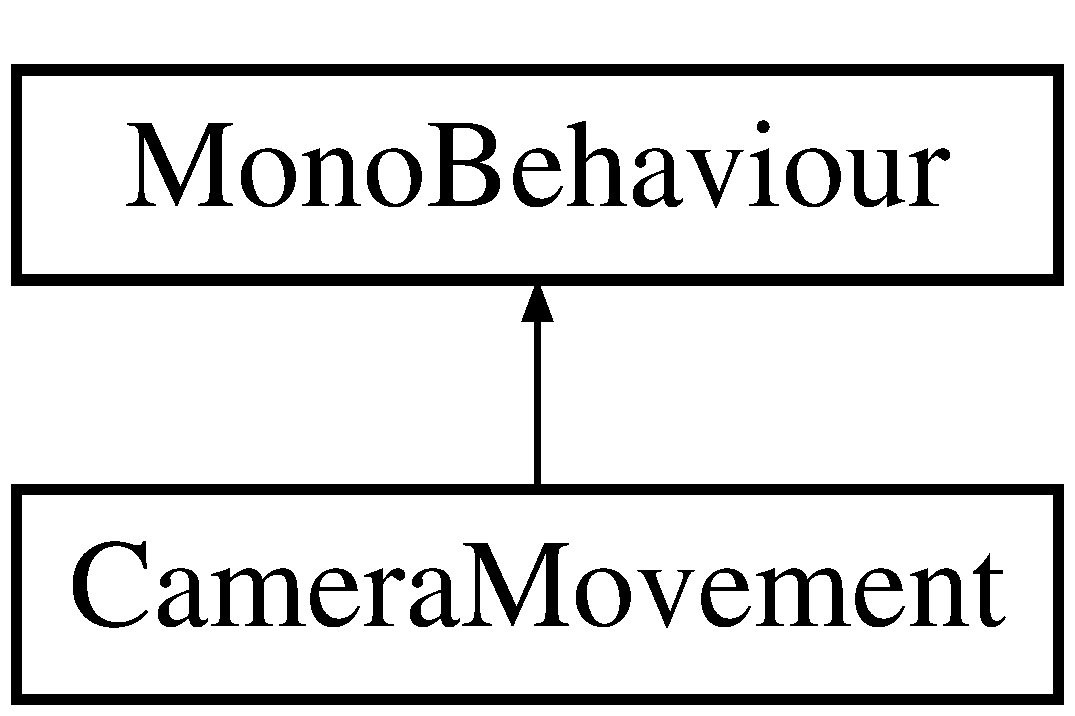
\includegraphics[height=2.000000cm]{class_camera_movement}
\end{center}
\end{figure}
\subsection*{Public Attributes}
\begin{DoxyCompactItemize}
\item 
\mbox{\Hypertarget{class_camera_movement_ab0c3a10c369ffb355282c53bf8e25fc1}\label{class_camera_movement_ab0c3a10c369ffb355282c53bf8e25fc1}} 
float \hyperlink{class_camera_movement_ab0c3a10c369ffb355282c53bf8e25fc1}{Scroll\+Speed} = 10f
\begin{DoxyCompactList}\small\item\em 
\begin{DoxyParams}{Parameters}
{\em Scroll\+Speed} & The speed at which scrolling/zooming in/out is executed when scrolling with the left mouse wheel.\\
\hline
\end{DoxyParams}
\end{DoxyCompactList}\item 
\mbox{\Hypertarget{class_camera_movement_ac23a09cdd06272b43e5090681e09095a}\label{class_camera_movement_ac23a09cdd06272b43e5090681e09095a}} 
float \hyperlink{class_camera_movement_ac23a09cdd06272b43e5090681e09095a}{Move\+Speed} = 0.\+1f
\begin{DoxyCompactList}\small\item\em 
\begin{DoxyParams}{Parameters}
{\em Move\+Speed} & The speed of the camera moving left/right and up/down when dragging with the move mouse button.\\
\hline
\end{DoxyParams}
\end{DoxyCompactList}\item 
\mbox{\Hypertarget{class_camera_movement_a0f6b3942fca01de3080b2728274ac102}\label{class_camera_movement_a0f6b3942fca01de3080b2728274ac102}} 
float \hyperlink{class_camera_movement_a0f6b3942fca01de3080b2728274ac102}{Rotate\+Speed} = 0.\+1f
\begin{DoxyCompactList}\small\item\em 
\begin{DoxyParams}{Parameters}
{\em Rotate\+Speed} & The speed of the camera rotating when dragging with the rotate mouse button.\\
\hline
\end{DoxyParams}
\end{DoxyCompactList}\end{DoxyCompactItemize}
\subsection*{Private Member Functions}
\begin{DoxyCompactItemize}
\item 
\mbox{\Hypertarget{class_camera_movement_a3d5bf0407152d0e16efafa655bfc15e9}\label{class_camera_movement_a3d5bf0407152d0e16efafa655bfc15e9}} 
void {\bfseries Start} ()
\item 
\mbox{\Hypertarget{class_camera_movement_a6d70b582440500fff98506ebd3e9050e}\label{class_camera_movement_a6d70b582440500fff98506ebd3e9050e}} 
void {\bfseries Update} ()
\end{DoxyCompactItemize}
\subsection*{Private Attributes}
\begin{DoxyCompactItemize}
\item 
\mbox{\Hypertarget{class_camera_movement_a68e2584501a6aaca0f1f4612d919da83}\label{class_camera_movement_a68e2584501a6aaca0f1f4612d919da83}} 
Vector3 \hyperlink{class_camera_movement_a68e2584501a6aaca0f1f4612d919da83}{Previous\+Mouse\+Position}
\begin{DoxyCompactList}\small\item\em 
\begin{DoxyParams}{Parameters}
{\em Previous\+Mouse\+Position} & Remembers the last mouse position since the last Update.\\
\hline
\end{DoxyParams}
\end{DoxyCompactList}\item 
\mbox{\Hypertarget{class_camera_movement_ae0a5e90a6fa1d305f2412d88e2bf2e35}\label{class_camera_movement_ae0a5e90a6fa1d305f2412d88e2bf2e35}} 
float \hyperlink{class_camera_movement_ae0a5e90a6fa1d305f2412d88e2bf2e35}{Yaw} = 0f
\begin{DoxyCompactList}\small\item\em 
\begin{DoxyParams}{Parameters}
{\em Yaw} & The yaw orientation of the camera.\\
\hline
\end{DoxyParams}
\end{DoxyCompactList}\item 
\mbox{\Hypertarget{class_camera_movement_adbf4bd21e962dbba99fdf24c85fc2665}\label{class_camera_movement_adbf4bd21e962dbba99fdf24c85fc2665}} 
float \hyperlink{class_camera_movement_adbf4bd21e962dbba99fdf24c85fc2665}{Pitch} = 0f
\begin{DoxyCompactList}\small\item\em 
\begin{DoxyParams}{Parameters}
{\em Pitch} & The pitch orientation of the camera.\\
\hline
\end{DoxyParams}
\end{DoxyCompactList}\end{DoxyCompactItemize}


\subsection{Detailed Description}
This class makes the camera draggable, rotatable and zoomable in the scene. 



The documentation for this class was generated from the following file\+:\begin{DoxyCompactItemize}
\item 
C\+:/\+Users/\+Mission\+Mankind/\+Desktop/\+Scripts/Camera\+Movement.\+cs\end{DoxyCompactItemize}

\hypertarget{class_extruder_updater}{}\section{Extruder\+Updater Class Reference}
\label{class_extruder_updater}\index{Extruder\+Updater@{Extruder\+Updater}}


This class updates the extruder needle location in the scene.  


Inheritance diagram for Extruder\+Updater\+:\begin{figure}[H]
\begin{center}
\leavevmode
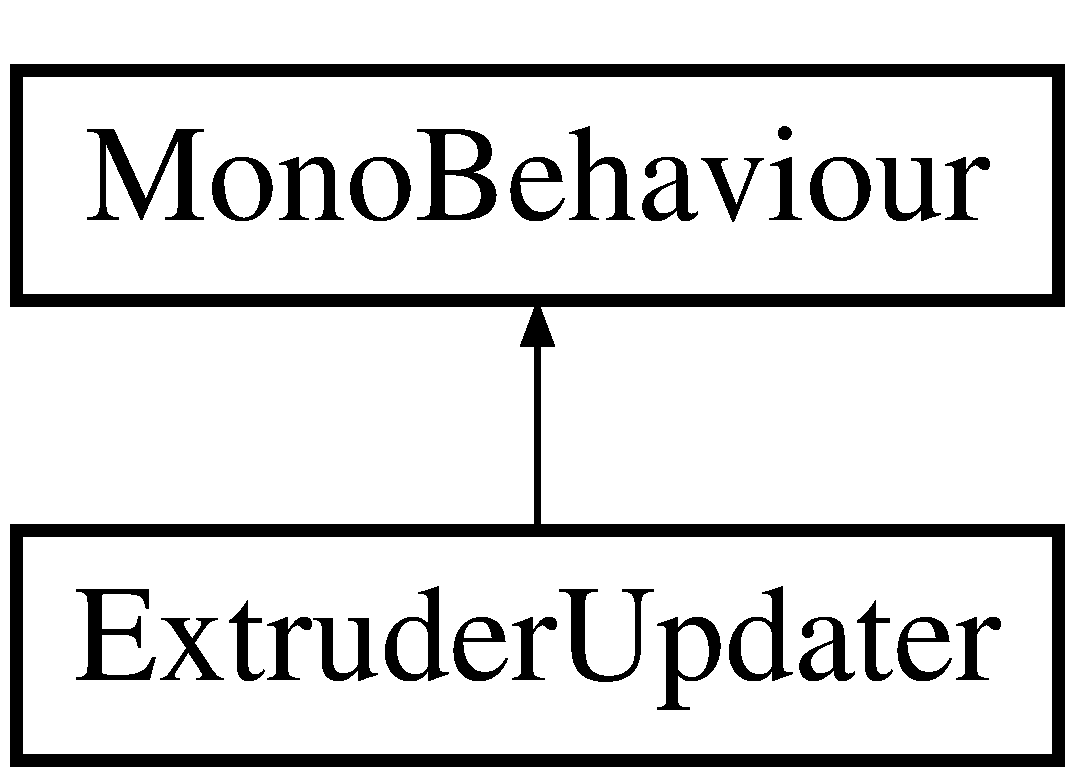
\includegraphics[height=2.000000cm]{class_extruder_updater}
\end{center}
\end{figure}
\subsection*{Private Member Functions}
\begin{DoxyCompactItemize}
\item 
\mbox{\Hypertarget{class_extruder_updater_ade597152d45f237ee471cacefa33ea26}\label{class_extruder_updater_ade597152d45f237ee471cacefa33ea26}} 
void {\bfseries Awake} ()
\item 
\mbox{\Hypertarget{class_extruder_updater_a514efae7cd29b947bb7ff5ffa1328875}\label{class_extruder_updater_a514efae7cd29b947bb7ff5ffa1328875}} 
void {\bfseries Update} ()
\end{DoxyCompactItemize}
\subsection*{Private Attributes}
\begin{DoxyCompactItemize}
\item 
\mbox{\Hypertarget{class_extruder_updater_a5e88f8bf7b9b76c903b7171af14daea5}\label{class_extruder_updater_a5e88f8bf7b9b76c903b7171af14daea5}} 
\hyperlink{class_printer}{Printer} \hyperlink{class_extruder_updater_a5e88f8bf7b9b76c903b7171af14daea5}{Printer}
\begin{DoxyCompactList}\small\item\em 
\begin{DoxyParams}{Parameters}
{\em \hyperlink{class_printer}{Printer}} & Object of the \hyperlink{class_printer}{Printer} that is used to request the printer needle location.\\
\hline
\end{DoxyParams}
\end{DoxyCompactList}\end{DoxyCompactItemize}


\subsection{Detailed Description}
This class updates the extruder needle location in the scene. 



The documentation for this class was generated from the following file\+:\begin{DoxyCompactItemize}
\item 
C\+:/\+Users/\+Mission\+Mankind/\+Desktop/\+Scripts/Extruder\+Updater.\+cs\end{DoxyCompactItemize}

\hypertarget{class_filament_manager}{}\section{Filament\+Manager Class Reference}
\label{class_filament_manager}\index{Filament\+Manager@{Filament\+Manager}}


The filament manager manages the spawning of filement meshes in the scene.  


Inheritance diagram for Filament\+Manager\+:\begin{figure}[H]
\begin{center}
\leavevmode
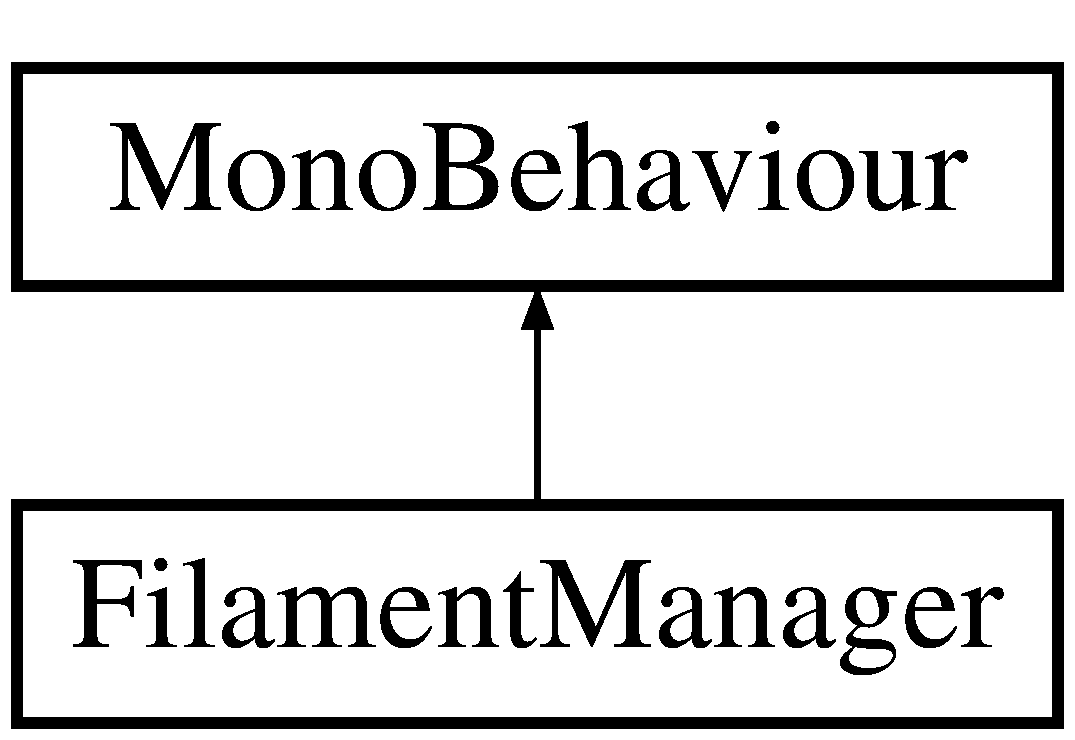
\includegraphics[height=2.000000cm]{class_filament_manager}
\end{center}
\end{figure}
\subsection*{Public Member Functions}
\begin{DoxyCompactItemize}
\item 
void \hyperlink{class_filament_manager_afda4accf27e892725d2a9974607421b6}{Add\+Filament} (Vector3 from, Vector3 to, float thickness)
\begin{DoxyCompactList}\small\item\em Adds a piece of filament to the simulation \end{DoxyCompactList}\end{DoxyCompactItemize}
\subsection*{Private Member Functions}
\begin{DoxyCompactItemize}
\item 
\mbox{\Hypertarget{class_filament_manager_ab870c17f0e1e66687fb56bfc46e9c2be}\label{class_filament_manager_ab870c17f0e1e66687fb56bfc46e9c2be}} 
void {\bfseries Start} ()
\item 
void \hyperlink{class_filament_manager_a088bc0f0147322c2970612c3b535cc3f}{Combine\+Temp} ()
\begin{DoxyCompactList}\small\item\em Combines all temporary objects into a single mesh \end{DoxyCompactList}\end{DoxyCompactItemize}
\subsection*{Private Attributes}
\begin{DoxyCompactItemize}
\item 
\mbox{\Hypertarget{class_filament_manager_a5e5d2ab663216f296edbf4b408c77b10}\label{class_filament_manager_a5e5d2ab663216f296edbf4b408c77b10}} 
Game\+Object \hyperlink{class_filament_manager_a5e5d2ab663216f296edbf4b408c77b10}{Empty\+Filament}
\begin{DoxyCompactList}\small\item\em 
\begin{DoxyParams}{Parameters}
{\em Empty\+Filament} & This object is used to add an empty mesh object to the scene. This object is then used to combine filament into one mesh.\\
\hline
\end{DoxyParams}
\end{DoxyCompactList}\item 
\mbox{\Hypertarget{class_filament_manager_ae127047f9f8d605818d2543182b9967a}\label{class_filament_manager_ae127047f9f8d605818d2543182b9967a}} 
Mesh \hyperlink{class_filament_manager_ae127047f9f8d605818d2543182b9967a}{Filament\+Mesh}
\begin{DoxyCompactList}\small\item\em 
\begin{DoxyParams}{Parameters}
{\em Filament\+Mesh} & This object is used to make a copy from the filament mesh resource.\\
\hline
\end{DoxyParams}
\end{DoxyCompactList}\item 
\mbox{\Hypertarget{class_filament_manager_a8a828b6fbdf60b77008801299aa6c71d}\label{class_filament_manager_a8a828b6fbdf60b77008801299aa6c71d}} 
int \hyperlink{class_filament_manager_a8a828b6fbdf60b77008801299aa6c71d}{Vertices\+Per\+Mesh}
\begin{DoxyCompactList}\small\item\em 
\begin{DoxyParams}{Parameters}
{\em Vertices\+Per\+Mesh} & Amount of vertices in the filament mesh.\\
\hline
\end{DoxyParams}
\end{DoxyCompactList}\item 
\mbox{\Hypertarget{class_filament_manager_a9401bd69ba21204265cd78a9a94e5b25}\label{class_filament_manager_a9401bd69ba21204265cd78a9a94e5b25}} 
int \hyperlink{class_filament_manager_a9401bd69ba21204265cd78a9a94e5b25}{Max\+Vertices\+Per\+Mesh} = 65536
\begin{DoxyCompactList}\small\item\em 
\begin{DoxyParams}{Parameters}
{\em Max\+Vertices\+Per\+Mesh} & Maximum number of vertices allowed in a Unity mesh (16 bit).\\
\hline
\end{DoxyParams}
\end{DoxyCompactList}\item 
\mbox{\Hypertarget{class_filament_manager_af7195c81156bf891185196a90f6459ca}\label{class_filament_manager_af7195c81156bf891185196a90f6459ca}} 
int \hyperlink{class_filament_manager_af7195c81156bf891185196a90f6459ca}{Filaments\+Per\+Mesh}
\begin{DoxyCompactList}\small\item\em 
\begin{DoxyParams}{Parameters}
{\em Filaments\+Per\+Mesh} & The amount of filaments that fit in a single mesh (Max\+Vertices\+Per\+Mesh / Vertices\+Per\+Mesh).\\
\hline
\end{DoxyParams}
\end{DoxyCompactList}\item 
\mbox{\Hypertarget{class_filament_manager_ac2355633fcdba276a7759483288e2555}\label{class_filament_manager_ac2355633fcdba276a7759483288e2555}} 
List$<$ Game\+Object $>$ \hyperlink{class_filament_manager_ac2355633fcdba276a7759483288e2555}{Objects}
\begin{DoxyCompactList}\small\item\em 
\begin{DoxyParams}{Parameters}
{\em Objects} & The objects containing the combined meshes.\\
\hline
\end{DoxyParams}
\end{DoxyCompactList}\item 
\mbox{\Hypertarget{class_filament_manager_a22596f86cb407fa0a91b7c3118ea2284}\label{class_filament_manager_a22596f86cb407fa0a91b7c3118ea2284}} 
Game\+Object \mbox{[}$\,$\mbox{]} \hyperlink{class_filament_manager_a22596f86cb407fa0a91b7c3118ea2284}{Temp\+Objects}
\begin{DoxyCompactList}\small\item\em 
\begin{DoxyParams}{Parameters}
{\em Temp\+Objects} & List of temporary gameobjects.\\
\hline
\end{DoxyParams}
\end{DoxyCompactList}\item 
\mbox{\Hypertarget{class_filament_manager_ae8591a3fbaae0dffffd99eb1ffd6416f}\label{class_filament_manager_ae8591a3fbaae0dffffd99eb1ffd6416f}} 
int \hyperlink{class_filament_manager_ae8591a3fbaae0dffffd99eb1ffd6416f}{Max\+Temp\+Objects} = 2500
\begin{DoxyCompactList}\small\item\em 
\begin{DoxyParams}{Parameters}
{\em Max\+Temp\+Objects} & Maximum number of temporary gameobjects until they are combined.\\
\hline
\end{DoxyParams}
\end{DoxyCompactList}\item 
\mbox{\Hypertarget{class_filament_manager_a9608a8f52bbfa6090658273943af3168}\label{class_filament_manager_a9608a8f52bbfa6090658273943af3168}} 
int \hyperlink{class_filament_manager_a9608a8f52bbfa6090658273943af3168}{Temp\+Index} = 0
\begin{DoxyCompactList}\small\item\em 
\begin{DoxyParams}{Parameters}
{\em Temp\+Index} & Index to store temporary object.\\
\hline
\end{DoxyParams}
\end{DoxyCompactList}\item 
\mbox{\Hypertarget{class_filament_manager_a783a989e028c64956987bfb3ca55c782}\label{class_filament_manager_a783a989e028c64956987bfb3ca55c782}} 
int \hyperlink{class_filament_manager_a783a989e028c64956987bfb3ca55c782}{Filament\+Count} = 0
\begin{DoxyCompactList}\small\item\em 
\begin{DoxyParams}{Parameters}
{\em Filament\+Count} & Amount of filaments created.\\
\hline
\end{DoxyParams}
\end{DoxyCompactList}\item 
\mbox{\Hypertarget{class_filament_manager_a209bee6c4f118778aa221fa7642c185f}\label{class_filament_manager_a209bee6c4f118778aa221fa7642c185f}} 
Vector3 \hyperlink{class_filament_manager_a209bee6c4f118778aa221fa7642c185f}{Previous\+From}
\begin{DoxyCompactList}\small\item\em 
\begin{DoxyParams}{Parameters}
{\em Filament\+Count} & Location of the previous filament, when a new object is added at the same location, it will extend the old.\\
\hline
\end{DoxyParams}
\end{DoxyCompactList}\item 
\mbox{\Hypertarget{class_filament_manager_a0b66beb7f8c31aee2c3c03c2917129b4}\label{class_filament_manager_a0b66beb7f8c31aee2c3c03c2917129b4}} 
const string {\bfseries Grouped\+Filament\+Name} = \char`\"{}Grouped\+Filament\char`\"{}
\end{DoxyCompactItemize}
\subsection*{Static Private Attributes}
\begin{DoxyCompactItemize}
\item 
\mbox{\Hypertarget{class_filament_manager_a0701818c4123f615adeb651037cec8cb}\label{class_filament_manager_a0701818c4123f615adeb651037cec8cb}} 
static Vector3 \hyperlink{class_filament_manager_a0701818c4123f615adeb651037cec8cb}{Totally\+Random} = new Vector3(39642f, 43785f, 325346f)
\begin{DoxyCompactList}\small\item\em 
\begin{DoxyParams}{Parameters}
{\em Totally\+Random} & Random vector to unset Previous\+From (Vector3 can\textquotesingle{}t be set to null).\\
\hline
\end{DoxyParams}
\end{DoxyCompactList}\end{DoxyCompactItemize}


\subsection{Detailed Description}
The filament manager manages the spawning of filement meshes in the scene. 



\subsection{Member Function Documentation}
\mbox{\Hypertarget{class_filament_manager_afda4accf27e892725d2a9974607421b6}\label{class_filament_manager_afda4accf27e892725d2a9974607421b6}} 
\index{Filament\+Manager@{Filament\+Manager}!Add\+Filament@{Add\+Filament}}
\index{Add\+Filament@{Add\+Filament}!Filament\+Manager@{Filament\+Manager}}
\subsubsection{\texorpdfstring{Add\+Filament()}{AddFilament()}}
{\footnotesize\ttfamily void Filament\+Manager.\+Add\+Filament (\begin{DoxyParamCaption}\item[{Vector3}]{from,  }\item[{Vector3}]{to,  }\item[{float}]{thickness }\end{DoxyParamCaption})}



Adds a piece of filament to the simulation 


\begin{DoxyParams}{Parameters}
{\em from} & Start position\\
\hline
{\em to} & End position\\
\hline
{\em thickness} & Radius of the thickness of the filament\\
\hline
\end{DoxyParams}
\mbox{\Hypertarget{class_filament_manager_a088bc0f0147322c2970612c3b535cc3f}\label{class_filament_manager_a088bc0f0147322c2970612c3b535cc3f}} 
\index{Filament\+Manager@{Filament\+Manager}!Combine\+Temp@{Combine\+Temp}}
\index{Combine\+Temp@{Combine\+Temp}!Filament\+Manager@{Filament\+Manager}}
\subsubsection{\texorpdfstring{Combine\+Temp()}{CombineTemp()}}
{\footnotesize\ttfamily void Filament\+Manager.\+Combine\+Temp (\begin{DoxyParamCaption}{ }\end{DoxyParamCaption})\hspace{0.3cm}{\ttfamily [private]}}



Combines all temporary objects into a single mesh 



The documentation for this class was generated from the following file\+:\begin{DoxyCompactItemize}
\item 
C\+:/\+Users/\+Mission\+Mankind/\+Desktop/\+Scripts/Filament\+Manager.\+cs\end{DoxyCompactItemize}

\hypertarget{class_gcode_command}{}\section{Gcode\+Command Class Reference}
\label{class_gcode_command}\index{Gcode\+Command@{Gcode\+Command}}


This class stores a single gcode command.  


\subsection*{Public Member Functions}
\begin{DoxyCompactItemize}
\item 
\hyperlink{class_gcode_command_aefd8e6144be3153471b2ee5e5fc500de}{Gcode\+Command} (string text)
\begin{DoxyCompactList}\small\item\em This constructor will convert a string of text into a \hyperlink{class_gcode_command}{Gcode\+Command} object if a single gcode command represents the text. \end{DoxyCompactList}\item 
bool \hyperlink{class_gcode_command_a21ddb89f360e9a2497855064cda0672a}{Is\+Valid} ()
\begin{DoxyCompactList}\small\item\em Returns true if a valid \hyperlink{class_gcode_command}{Gcode\+Command} has been initialized. \end{DoxyCompactList}\item 
int \hyperlink{class_gcode_command_ad40c68e4595b030959155c66fb66f154}{Get\+Command\+Type} ()
\begin{DoxyCompactList}\small\item\em This function gives back the type of \hyperlink{class_gcode_command}{Gcode\+Command}. \end{DoxyCompactList}\end{DoxyCompactItemize}
\subsection*{Public Attributes}
\begin{DoxyCompactItemize}
\item 
\mbox{\Hypertarget{class_gcode_command_a5b7b9c6bd1f4e1f1ecbace62f323ca72}\label{class_gcode_command_a5b7b9c6bd1f4e1f1ecbace62f323ca72}} 
float \hyperlink{class_gcode_command_a5b7b9c6bd1f4e1f1ecbace62f323ca72}{X} = G\+Mcodes.\+Invalid\+Number
\begin{DoxyCompactList}\small\item\em 
\begin{DoxyParams}{Parameters}
{\em X} & This float is one of the possible parameters for a single G-\/code command.\\
\hline
\end{DoxyParams}
\end{DoxyCompactList}\item 
\mbox{\Hypertarget{class_gcode_command_a27525d0b7ae679a68bee5900fb76b591}\label{class_gcode_command_a27525d0b7ae679a68bee5900fb76b591}} 
float \hyperlink{class_gcode_command_a27525d0b7ae679a68bee5900fb76b591}{Y} = G\+Mcodes.\+Invalid\+Number
\begin{DoxyCompactList}\small\item\em 
\begin{DoxyParams}{Parameters}
{\em Y} & This float is one of the possible parameters for a single G-\/code command.\\
\hline
\end{DoxyParams}
\end{DoxyCompactList}\item 
\mbox{\Hypertarget{class_gcode_command_aa6f11f780ad151a1c233b65873369fd6}\label{class_gcode_command_aa6f11f780ad151a1c233b65873369fd6}} 
float \hyperlink{class_gcode_command_aa6f11f780ad151a1c233b65873369fd6}{Z} = G\+Mcodes.\+Invalid\+Number
\begin{DoxyCompactList}\small\item\em 
\begin{DoxyParams}{Parameters}
{\em Z} & This float is one of the possible parameters for a single G-\/code command.\\
\hline
\end{DoxyParams}
\end{DoxyCompactList}\item 
\mbox{\Hypertarget{class_gcode_command_ad853d24d1bd2f9a240db21073aa70485}\label{class_gcode_command_ad853d24d1bd2f9a240db21073aa70485}} 
float \hyperlink{class_gcode_command_ad853d24d1bd2f9a240db21073aa70485}{E} = G\+Mcodes.\+Invalid\+Number
\begin{DoxyCompactList}\small\item\em 
\begin{DoxyParams}{Parameters}
{\em E} & This float is one of the possible parameters for a single G-\/code command.\\
\hline
\end{DoxyParams}
\end{DoxyCompactList}\item 
\mbox{\Hypertarget{class_gcode_command_a93dd15b57d51fa236b9ff7451fab7869}\label{class_gcode_command_a93dd15b57d51fa236b9ff7451fab7869}} 
float \hyperlink{class_gcode_command_a93dd15b57d51fa236b9ff7451fab7869}{F} = G\+Mcodes.\+Invalid\+Number
\begin{DoxyCompactList}\small\item\em 
\begin{DoxyParams}{Parameters}
{\em F} & This float is one of the possible parameters for a single G-\/code command.\\
\hline
\end{DoxyParams}
\end{DoxyCompactList}\item 
\mbox{\Hypertarget{class_gcode_command_a3cddf7beda991f104e128f5caee224f1}\label{class_gcode_command_a3cddf7beda991f104e128f5caee224f1}} 
float \hyperlink{class_gcode_command_a3cddf7beda991f104e128f5caee224f1}{S} = G\+Mcodes.\+Invalid\+Number
\begin{DoxyCompactList}\small\item\em 
\begin{DoxyParams}{Parameters}
{\em S} & This float is one of the possible parameters for a single G-\/code command.\\
\hline
\end{DoxyParams}
\end{DoxyCompactList}\end{DoxyCompactItemize}
\subsection*{Private Member Functions}
\begin{DoxyCompactItemize}
\item 
List$<$ string $>$ \hyperlink{class_gcode_command_a39d602bf1f22666bc0dd2431b15214ed}{Number\+Split} (string text)
\begin{DoxyCompactList}\small\item\em This function converts a string to a List of floating numbers that are still in string form. \end{DoxyCompactList}\end{DoxyCompactItemize}
\subsection*{Static Private Member Functions}
\begin{DoxyCompactItemize}
\item 
static float \hyperlink{class_gcode_command_a7e60f42effcf4a0053d812e16ffa3895}{String\+To\+Float} (string input)
\begin{DoxyCompactList}\small\item\em An optimized string to float conversion method, without error checking. \end{DoxyCompactList}\end{DoxyCompactItemize}
\subsection*{Private Attributes}
\begin{DoxyCompactItemize}
\item 
\mbox{\Hypertarget{class_gcode_command_acd40d4810d479c4913f7958d75356bbe}\label{class_gcode_command_acd40d4810d479c4913f7958d75356bbe}} 
int \hyperlink{class_gcode_command_acd40d4810d479c4913f7958d75356bbe}{Type}
\begin{DoxyCompactList}\small\item\em 
\begin{DoxyParams}{Parameters}
{\em Type} & Contains the value identified the type of G-\/code command.\\
\hline
\end{DoxyParams}
\end{DoxyCompactList}\item 
\mbox{\Hypertarget{class_gcode_command_a958029bcc2cc71475f99bee849182a47}\label{class_gcode_command_a958029bcc2cc71475f99bee849182a47}} 
bool \hyperlink{class_gcode_command_a958029bcc2cc71475f99bee849182a47}{Valid} = true
\begin{DoxyCompactList}\small\item\em 
\begin{DoxyParams}{Parameters}
{\em Valid} & Boolean that represenents true if this is a valid G-\/code command.\\
\hline
\end{DoxyParams}
\end{DoxyCompactList}\end{DoxyCompactItemize}


\subsection{Detailed Description}
This class stores a single gcode command. 



\subsection{Constructor \& Destructor Documentation}
\mbox{\Hypertarget{class_gcode_command_aefd8e6144be3153471b2ee5e5fc500de}\label{class_gcode_command_aefd8e6144be3153471b2ee5e5fc500de}} 
\index{Gcode\+Command@{Gcode\+Command}!Gcode\+Command@{Gcode\+Command}}
\index{Gcode\+Command@{Gcode\+Command}!Gcode\+Command@{Gcode\+Command}}
\subsubsection{\texorpdfstring{Gcode\+Command()}{GcodeCommand()}}
{\footnotesize\ttfamily Gcode\+Command.\+Gcode\+Command (\begin{DoxyParamCaption}\item[{string}]{text }\end{DoxyParamCaption})}



This constructor will convert a string of text into a \hyperlink{class_gcode_command}{Gcode\+Command} object if a single gcode command represents the text. 


\begin{DoxyParams}{Parameters}
{\em text} & The line of text representing a single gcode command. Example\+: \char`\"{}\+G1 X1.\+27 Y5.\+44 Z5.\+55 E0.\+44 F400.\+00\char`\"{}\\
\hline
\end{DoxyParams}


\subsection{Member Function Documentation}
\mbox{\Hypertarget{class_gcode_command_ad40c68e4595b030959155c66fb66f154}\label{class_gcode_command_ad40c68e4595b030959155c66fb66f154}} 
\index{Gcode\+Command@{Gcode\+Command}!Get\+Command\+Type@{Get\+Command\+Type}}
\index{Get\+Command\+Type@{Get\+Command\+Type}!Gcode\+Command@{Gcode\+Command}}
\subsubsection{\texorpdfstring{Get\+Command\+Type()}{GetCommandType()}}
{\footnotesize\ttfamily int Gcode\+Command.\+Get\+Command\+Type (\begin{DoxyParamCaption}{ }\end{DoxyParamCaption})}



This function gives back the type of \hyperlink{class_gcode_command}{Gcode\+Command}. 

\begin{DoxyReturn}{Returns}
Returns the type of \hyperlink{class_gcode_command}{Gcode\+Command}. This type determines what type of action the gcode command is.
\end{DoxyReturn}
\mbox{\Hypertarget{class_gcode_command_a21ddb89f360e9a2497855064cda0672a}\label{class_gcode_command_a21ddb89f360e9a2497855064cda0672a}} 
\index{Gcode\+Command@{Gcode\+Command}!Is\+Valid@{Is\+Valid}}
\index{Is\+Valid@{Is\+Valid}!Gcode\+Command@{Gcode\+Command}}
\subsubsection{\texorpdfstring{Is\+Valid()}{IsValid()}}
{\footnotesize\ttfamily bool Gcode\+Command.\+Is\+Valid (\begin{DoxyParamCaption}{ }\end{DoxyParamCaption})}



Returns true if a valid \hyperlink{class_gcode_command}{Gcode\+Command} has been initialized. 

\begin{DoxyReturn}{Returns}
The boolean containing if the \hyperlink{class_gcode_command}{Gcode\+Command} has been initialized if true, otherwise false.
\end{DoxyReturn}
\mbox{\Hypertarget{class_gcode_command_a39d602bf1f22666bc0dd2431b15214ed}\label{class_gcode_command_a39d602bf1f22666bc0dd2431b15214ed}} 
\index{Gcode\+Command@{Gcode\+Command}!Number\+Split@{Number\+Split}}
\index{Number\+Split@{Number\+Split}!Gcode\+Command@{Gcode\+Command}}
\subsubsection{\texorpdfstring{Number\+Split()}{NumberSplit()}}
{\footnotesize\ttfamily List$<$string$>$ Gcode\+Command.\+Number\+Split (\begin{DoxyParamCaption}\item[{string}]{text }\end{DoxyParamCaption})\hspace{0.3cm}{\ttfamily [private]}}



This function converts a string to a List of floating numbers that are still in string form. 


\begin{DoxyParams}{Parameters}
{\em text} & The input text that will be converted.\\
\hline
\end{DoxyParams}
\begin{DoxyReturn}{Returns}
Returns the list of numbers that were split from the input text.
\end{DoxyReturn}
\mbox{\Hypertarget{class_gcode_command_a7e60f42effcf4a0053d812e16ffa3895}\label{class_gcode_command_a7e60f42effcf4a0053d812e16ffa3895}} 
\index{Gcode\+Command@{Gcode\+Command}!String\+To\+Float@{String\+To\+Float}}
\index{String\+To\+Float@{String\+To\+Float}!Gcode\+Command@{Gcode\+Command}}
\subsubsection{\texorpdfstring{String\+To\+Float()}{StringToFloat()}}
{\footnotesize\ttfamily static float Gcode\+Command.\+String\+To\+Float (\begin{DoxyParamCaption}\item[{string}]{input }\end{DoxyParamCaption})\hspace{0.3cm}{\ttfamily [static]}, {\ttfamily [private]}}



An optimized string to float conversion method, without error checking. 


\begin{DoxyParams}{Parameters}
{\em input} & The string that will be converted to the float.\\
\hline
\end{DoxyParams}
\begin{DoxyReturn}{Returns}
Returns the resulting float from the string input.
\end{DoxyReturn}


The documentation for this class was generated from the following file\+:\begin{DoxyCompactItemize}
\item 
C\+:/\+Users/\+Mission\+Mankind/\+Desktop/\+Scripts/Gcode\+Command.\+cs\end{DoxyCompactItemize}

\hypertarget{class_gcode_loader}{}\section{Gcode\+Loader Class Reference}
\label{class_gcode_loader}\index{Gcode\+Loader@{Gcode\+Loader}}


The \hyperlink{class_gcode_loader}{Gcode\+Loader} loads gcode from a file into memory. It is also used to loop through the gcode commands to let the \hyperlink{class_printer}{Printer} class execute the commands.  


\subsection*{Public Member Functions}
\begin{DoxyCompactItemize}
\item 
bool \hyperlink{class_gcode_loader_a295f2e6de27384942c01024adf7a0615}{Execute\+Next\+Command} (\hyperlink{class_printer}{Printer} printer)
\begin{DoxyCompactList}\small\item\em Handles moving to the new Gcode command and then calls another function to execute the command for the \hyperlink{class_printer}{Printer} object. \end{DoxyCompactList}\item 
bool \hyperlink{class_gcode_loader_a6b8aedf9e1c0b90d931626697bc9c3de}{End\+Of\+Gcode} ()
\begin{DoxyCompactList}\small\item\em Returns true if the end of the gcode has been reached. \end{DoxyCompactList}\item 
void \hyperlink{class_gcode_loader_a921de7da9cc2e377a52977f30f8c1204}{Load} (string filename)
\begin{DoxyCompactList}\small\item\em Loads all gcode from a file into memory and links all variables in the gcode into a structured class. \end{DoxyCompactList}\end{DoxyCompactItemize}
\subsection*{Public Attributes}
\begin{DoxyCompactItemize}
\item 
\mbox{\Hypertarget{class_gcode_loader_a5c5558ee51ad2dc684951b4e69e95112}\label{class_gcode_loader_a5c5558ee51ad2dc684951b4e69e95112}} 
bool \hyperlink{class_gcode_loader_a5c5558ee51ad2dc684951b4e69e95112}{Model\+Loaded} = false
\begin{DoxyCompactList}\small\item\em 
\begin{DoxyParams}{Parameters}
{\em Model\+Loaded} & Boolean representing if a model has already been loaded into the gcode.\\
\hline
\end{DoxyParams}
\end{DoxyCompactList}\end{DoxyCompactItemize}
\subsection*{Private Member Functions}
\begin{DoxyCompactItemize}
\item 
void \hyperlink{class_gcode_loader_a82cfb2c8e208446db42b8d570bf9bc85}{Execute\+Command} (\hyperlink{class_gcode_command}{Gcode\+Command} command, \hyperlink{class_printer}{Printer} printer)
\begin{DoxyCompactList}\small\item\em Determines the command to execute and then calls the matching function with parameters to the \hyperlink{class_printer}{Printer} object. \end{DoxyCompactList}\item 
void \hyperlink{class_gcode_loader_a4022243922bb02571c83a4f0897bc45f}{Load} (string filename, List$<$ \hyperlink{class_gcode_command}{Gcode\+Command} $>$ new\+Commands)
\begin{DoxyCompactList}\small\item\em Loads all gcode from a file into memory and links all variables in the gcode into a structured class. \end{DoxyCompactList}\end{DoxyCompactItemize}
\subsection*{Private Attributes}
\begin{DoxyCompactItemize}
\item 
\mbox{\Hypertarget{class_gcode_loader_a61536e92fe75a3387758adb23c915dd7}\label{class_gcode_loader_a61536e92fe75a3387758adb23c915dd7}} 
List$<$ \hyperlink{class_gcode_command}{Gcode\+Command} $>$ \hyperlink{class_gcode_loader_a61536e92fe75a3387758adb23c915dd7}{Commands} = new List$<$\hyperlink{class_gcode_command}{Gcode\+Command}$>$()
\begin{DoxyCompactList}\small\item\em 
\begin{DoxyParams}{Parameters}
{\em Commands} & A list containing all gcode commands.\\
\hline
\end{DoxyParams}
\end{DoxyCompactList}\item 
\mbox{\Hypertarget{class_gcode_loader_a4d184919835f2dfb469887d83b464c82}\label{class_gcode_loader_a4d184919835f2dfb469887d83b464c82}} 
int \hyperlink{class_gcode_loader_a4d184919835f2dfb469887d83b464c82}{Commands\+Index} = 0
\begin{DoxyCompactList}\small\item\em 
\begin{DoxyParams}{Parameters}
{\em Commands\+Index} & The current index of the last read gcode command. Used for the Next\+Gcode\+Command function.\\
\hline
\end{DoxyParams}
\end{DoxyCompactList}\end{DoxyCompactItemize}


\subsection{Detailed Description}
The \hyperlink{class_gcode_loader}{Gcode\+Loader} loads gcode from a file into memory. It is also used to loop through the gcode commands to let the \hyperlink{class_printer}{Printer} class execute the commands. 



\subsection{Member Function Documentation}
\mbox{\Hypertarget{class_gcode_loader_a6b8aedf9e1c0b90d931626697bc9c3de}\label{class_gcode_loader_a6b8aedf9e1c0b90d931626697bc9c3de}} 
\index{Gcode\+Loader@{Gcode\+Loader}!End\+Of\+Gcode@{End\+Of\+Gcode}}
\index{End\+Of\+Gcode@{End\+Of\+Gcode}!Gcode\+Loader@{Gcode\+Loader}}
\subsubsection{\texorpdfstring{End\+Of\+Gcode()}{EndOfGcode()}}
{\footnotesize\ttfamily bool Gcode\+Loader.\+End\+Of\+Gcode (\begin{DoxyParamCaption}{ }\end{DoxyParamCaption})}



Returns true if the end of the gcode has been reached. 

\begin{DoxyReturn}{Returns}
Returns true if the \hyperlink{class_gcode_loader}{Gcode\+Loader} is at the end of the G-\/code file. Returns true otherwise.
\end{DoxyReturn}
\mbox{\Hypertarget{class_gcode_loader_a82cfb2c8e208446db42b8d570bf9bc85}\label{class_gcode_loader_a82cfb2c8e208446db42b8d570bf9bc85}} 
\index{Gcode\+Loader@{Gcode\+Loader}!Execute\+Command@{Execute\+Command}}
\index{Execute\+Command@{Execute\+Command}!Gcode\+Loader@{Gcode\+Loader}}
\subsubsection{\texorpdfstring{Execute\+Command()}{ExecuteCommand()}}
{\footnotesize\ttfamily void Gcode\+Loader.\+Execute\+Command (\begin{DoxyParamCaption}\item[{\hyperlink{class_gcode_command}{Gcode\+Command}}]{command,  }\item[{\hyperlink{class_printer}{Printer}}]{printer }\end{DoxyParamCaption})\hspace{0.3cm}{\ttfamily [private]}}



Determines the command to execute and then calls the matching function with parameters to the \hyperlink{class_printer}{Printer} object. 


\begin{DoxyParams}{Parameters}
{\em command} & The command object that will contain all information of the command.\\
\hline
{\em printer} & The printer object that requested a new command.\\
\hline
\end{DoxyParams}
\mbox{\Hypertarget{class_gcode_loader_a295f2e6de27384942c01024adf7a0615}\label{class_gcode_loader_a295f2e6de27384942c01024adf7a0615}} 
\index{Gcode\+Loader@{Gcode\+Loader}!Execute\+Next\+Command@{Execute\+Next\+Command}}
\index{Execute\+Next\+Command@{Execute\+Next\+Command}!Gcode\+Loader@{Gcode\+Loader}}
\subsubsection{\texorpdfstring{Execute\+Next\+Command()}{ExecuteNextCommand()}}
{\footnotesize\ttfamily bool Gcode\+Loader.\+Execute\+Next\+Command (\begin{DoxyParamCaption}\item[{\hyperlink{class_printer}{Printer}}]{printer }\end{DoxyParamCaption})}



Handles moving to the new Gcode command and then calls another function to execute the command for the \hyperlink{class_printer}{Printer} object. 


\begin{DoxyParams}{Parameters}
{\em printer} & The printer object that requested a new command.\\
\hline
\end{DoxyParams}
\begin{DoxyReturn}{Returns}
Returns false if end of G-\/code file or no model has been loaded. Returns true otherwise.
\end{DoxyReturn}
\mbox{\Hypertarget{class_gcode_loader_a921de7da9cc2e377a52977f30f8c1204}\label{class_gcode_loader_a921de7da9cc2e377a52977f30f8c1204}} 
\index{Gcode\+Loader@{Gcode\+Loader}!Load@{Load}}
\index{Load@{Load}!Gcode\+Loader@{Gcode\+Loader}}
\subsubsection{\texorpdfstring{Load()}{Load()}\hspace{0.1cm}{\footnotesize\ttfamily [1/2]}}
{\footnotesize\ttfamily void Gcode\+Loader.\+Load (\begin{DoxyParamCaption}\item[{string}]{filename }\end{DoxyParamCaption})}



Loads all gcode from a file into memory and links all variables in the gcode into a structured class. 


\begin{DoxyParams}{Parameters}
{\em filename} & The name of the file where to load the gcode from.\\
\hline
\end{DoxyParams}
\mbox{\Hypertarget{class_gcode_loader_a4022243922bb02571c83a4f0897bc45f}\label{class_gcode_loader_a4022243922bb02571c83a4f0897bc45f}} 
\index{Gcode\+Loader@{Gcode\+Loader}!Load@{Load}}
\index{Load@{Load}!Gcode\+Loader@{Gcode\+Loader}}
\subsubsection{\texorpdfstring{Load()}{Load()}\hspace{0.1cm}{\footnotesize\ttfamily [2/2]}}
{\footnotesize\ttfamily void Gcode\+Loader.\+Load (\begin{DoxyParamCaption}\item[{string}]{filename,  }\item[{List$<$ \hyperlink{class_gcode_command}{Gcode\+Command} $>$}]{new\+Commands }\end{DoxyParamCaption})\hspace{0.3cm}{\ttfamily [private]}}



Loads all gcode from a file into memory and links all variables in the gcode into a structured class. 


\begin{DoxyParams}{Parameters}
{\em filename} & The name of the file where to load the gcode from.\\
\hline
{\em new\+Commands} & The list where all gcode commands will be stored in.\\
\hline
\end{DoxyParams}


The documentation for this class was generated from the following file\+:\begin{DoxyCompactItemize}
\item 
C\+:/\+Users/\+Mission\+Mankind/\+Desktop/\+Scripts/Gcode\+Loader.\+cs\end{DoxyCompactItemize}

\hypertarget{class_g_mcodes}{}\section{G\+Mcodes Class Reference}
\label{class_g_mcodes}\index{G\+Mcodes@{G\+Mcodes}}


This class contains all values of the matching G and M codes.  


\subsection*{Public Attributes}
\begin{DoxyCompactItemize}
\item 
\mbox{\Hypertarget{class_g_mcodes_ad6e272392e966459b94901074a977ff3}\label{class_g_mcodes_ad6e272392e966459b94901074a977ff3}} 
const float {\bfseries Invalid\+Number} = -\/1000000000
\item 
\mbox{\Hypertarget{class_g_mcodes_ac4f23bb4a68aeb87380906a797ff5cd9}\label{class_g_mcodes_ac4f23bb4a68aeb87380906a797ff5cd9}} 
const int \hyperlink{class_g_mcodes_ac4f23bb4a68aeb87380906a797ff5cd9}{Move0} = 0
\begin{DoxyCompactList}\small\item\em 
\begin{DoxyParams}{Parameters}
{\em Move0} & The command for moving the printer with filament.\\
\hline
\end{DoxyParams}
\end{DoxyCompactList}\item 
\mbox{\Hypertarget{class_g_mcodes_a1b7866302ea84e792d4a0b202fca7572}\label{class_g_mcodes_a1b7866302ea84e792d4a0b202fca7572}} 
const int \hyperlink{class_g_mcodes_a1b7866302ea84e792d4a0b202fca7572}{Move1} = 1
\begin{DoxyCompactList}\small\item\em 
\begin{DoxyParams}{Parameters}
{\em Move1} & The command for moving the printer without filament.\\
\hline
\end{DoxyParams}
\end{DoxyCompactList}\item 
\mbox{\Hypertarget{class_g_mcodes_a8effe1399412977673f4a7d719d9f478}\label{class_g_mcodes_a8effe1399412977673f4a7d719d9f478}} 
const int \hyperlink{class_g_mcodes_a8effe1399412977673f4a7d719d9f478}{Home\+Axis} = 28
\begin{DoxyCompactList}\small\item\em 
\begin{DoxyParams}{Parameters}
{\em Home\+Axis} & A Move1 command at maximum speed to the home coordinates (0,0,0).\\
\hline
\end{DoxyParams}
\end{DoxyCompactList}\item 
\mbox{\Hypertarget{class_g_mcodes_aef9ced59d2c0feef2ec1caafd1a3d6f3}\label{class_g_mcodes_aef9ced59d2c0feef2ec1caafd1a3d6f3}} 
const int \hyperlink{class_g_mcodes_aef9ced59d2c0feef2ec1caafd1a3d6f3}{Set\+Extruder\+Temperature1} = 104
\begin{DoxyCompactList}\small\item\em 
\begin{DoxyParams}{Parameters}
{\em Set\+Extruder\+Temperature1} & Sets the extruder temperature for Rep\+Rap G-\/code.\\
\hline
\end{DoxyParams}
\end{DoxyCompactList}\item 
\mbox{\Hypertarget{class_g_mcodes_af52a427822185c005317834f84f351b9}\label{class_g_mcodes_af52a427822185c005317834f84f351b9}} 
const int \hyperlink{class_g_mcodes_af52a427822185c005317834f84f351b9}{Set\+Extruder\+Temperature2} = 109
\begin{DoxyCompactList}\small\item\em 
\begin{DoxyParams}{Parameters}
{\em Set\+Extruder\+Temperature2} & Sets the extruder temperature for Ulti\+G\+Code G-\/code.\\
\hline
\end{DoxyParams}
\end{DoxyCompactList}\item 
\mbox{\Hypertarget{class_g_mcodes_ada9741115088ea15e37ae8eda2fa8d9e}\label{class_g_mcodes_ada9741115088ea15e37ae8eda2fa8d9e}} 
const int \hyperlink{class_g_mcodes_ada9741115088ea15e37ae8eda2fa8d9e}{Set\+Bed\+Temperature1} = 140
\begin{DoxyCompactList}\small\item\em 
\begin{DoxyParams}{Parameters}
{\em Set\+Bed\+Temperature1} & Sets the bed temperature for Rep\+Rap G-\/code.\\
\hline
\end{DoxyParams}
\end{DoxyCompactList}\item 
\mbox{\Hypertarget{class_g_mcodes_ad64aba8e5361df2deb1a660988f0c4dc}\label{class_g_mcodes_ad64aba8e5361df2deb1a660988f0c4dc}} 
const int \hyperlink{class_g_mcodes_ad64aba8e5361df2deb1a660988f0c4dc}{Set\+Bed\+Temperature2} = 190
\begin{DoxyCompactList}\small\item\em 
\begin{DoxyParams}{Parameters}
{\em Set\+Bed\+Temperature2} & Sets the bed temperature for Ulti\+G\+Code G-\/code.\\
\hline
\end{DoxyParams}
\end{DoxyCompactList}\end{DoxyCompactItemize}


\subsection{Detailed Description}
This class contains all values of the matching G and M codes. 



The documentation for this class was generated from the following file\+:\begin{DoxyCompactItemize}
\item 
C\+:/\+Users/\+Mission\+Mankind/\+Desktop/\+Scripts/Gcodes.\+cs\end{DoxyCompactItemize}

\hypertarget{class_print_bed_updater}{}\section{Print\+Bed\+Updater Class Reference}
\label{class_print_bed_updater}\index{Print\+Bed\+Updater@{Print\+Bed\+Updater}}


This class updates the print bed location in the scene.  


Inheritance diagram for Print\+Bed\+Updater\+:\begin{figure}[H]
\begin{center}
\leavevmode
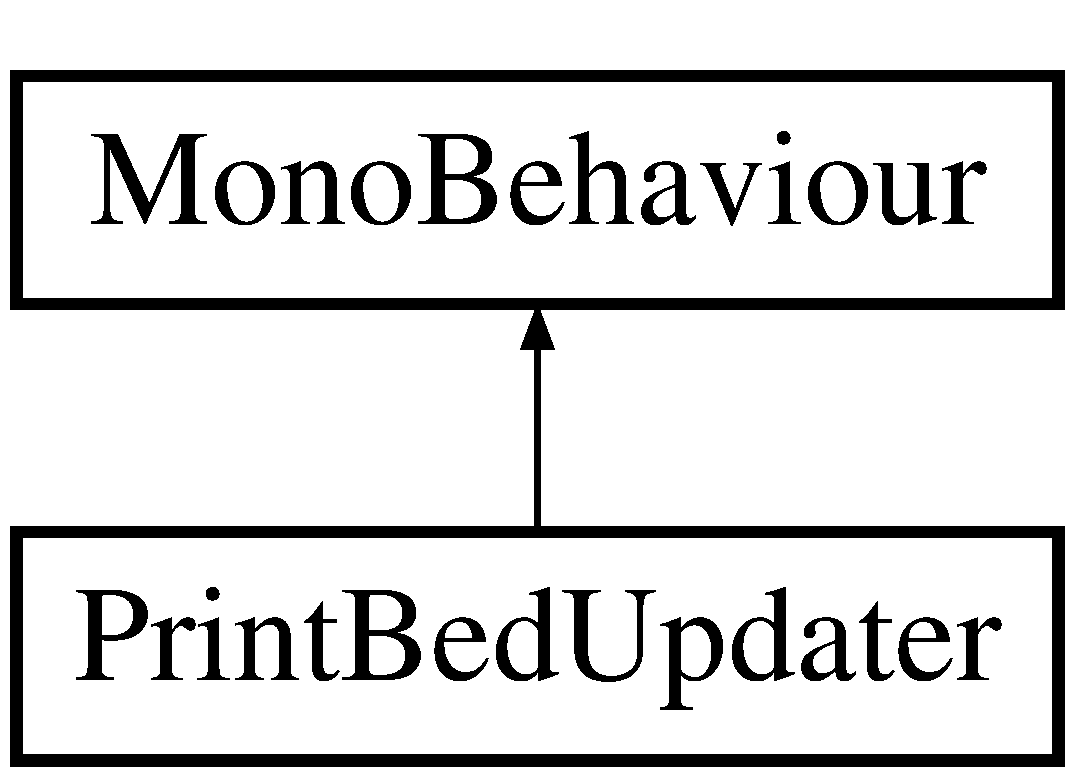
\includegraphics[height=2.000000cm]{class_print_bed_updater}
\end{center}
\end{figure}
\subsection*{Private Member Functions}
\begin{DoxyCompactItemize}
\item 
\mbox{\Hypertarget{class_print_bed_updater_a84c4921ef2706e2a253f8308c5f743e0}\label{class_print_bed_updater_a84c4921ef2706e2a253f8308c5f743e0}} 
void {\bfseries Awake} ()
\item 
\mbox{\Hypertarget{class_print_bed_updater_a9da635b8b219ecf5ce47dcb6a6febd40}\label{class_print_bed_updater_a9da635b8b219ecf5ce47dcb6a6febd40}} 
void {\bfseries Update} ()
\end{DoxyCompactItemize}
\subsection*{Private Attributes}
\begin{DoxyCompactItemize}
\item 
\mbox{\Hypertarget{class_print_bed_updater_a4a3f66dcbabccd470441a02ea463fe52}\label{class_print_bed_updater_a4a3f66dcbabccd470441a02ea463fe52}} 
\hyperlink{class_printer}{Printer} \hyperlink{class_print_bed_updater_a4a3f66dcbabccd470441a02ea463fe52}{Printer}
\begin{DoxyCompactList}\small\item\em 
\begin{DoxyParams}{Parameters}
{\em \hyperlink{class_printer}{Printer}} & Object of the \hyperlink{class_printer}{Printer} that is used to request the printer bed location.\\
\hline
\end{DoxyParams}
\end{DoxyCompactList}\end{DoxyCompactItemize}


\subsection{Detailed Description}
This class updates the print bed location in the scene. 



The documentation for this class was generated from the following file\+:\begin{DoxyCompactItemize}
\item 
C\+:/\+Users/\+Mission\+Mankind/\+Desktop/\+Scripts/Print\+Bed\+Updater.\+cs\end{DoxyCompactItemize}

\hypertarget{class_printer}{}\section{Printer Class Reference}
\label{class_printer}\index{Printer@{Printer}}


This class progresses the printprocess and is used as central control unit in executing G-\/code commands.  


Inheritance diagram for Printer\+:\begin{figure}[H]
\begin{center}
\leavevmode
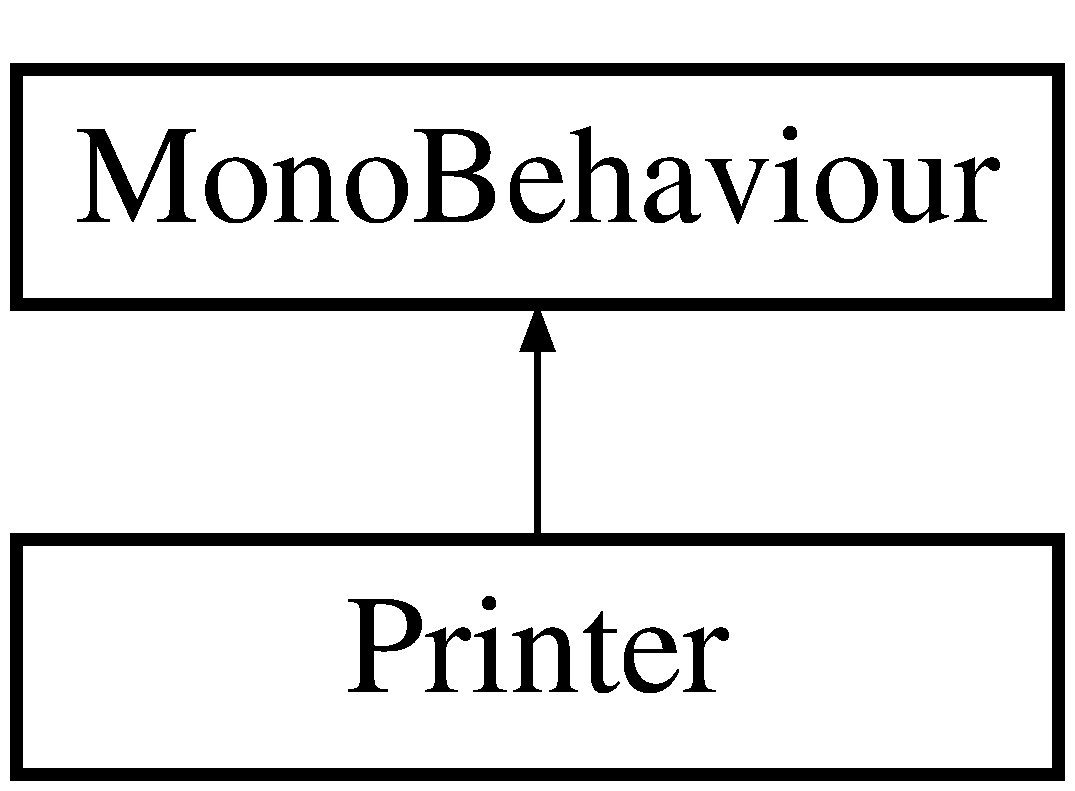
\includegraphics[height=2.000000cm]{class_printer}
\end{center}
\end{figure}
\subsection*{Public Member Functions}
\begin{DoxyCompactItemize}
\item 
void \hyperlink{class_printer_aca020f5d2c184af8ecdfd818577815bd}{Select\+File} ()
\begin{DoxyCompactList}\small\item\em This function is used to trigger a select window to choose a file from the filesystem that has G-\/code inside it. \end{DoxyCompactList}\item 
void \hyperlink{class_printer_ab90889903063563e05b7c6409a944752}{Set\+Time\+Multiplier} (float multiplier)
\begin{DoxyCompactList}\small\item\em This function sets the Time\+Multiplier. This param influences the simulation speed. \end{DoxyCompactList}\item 
void \hyperlink{class_printer_adfa651ad28cdcb1b26f135f32d414f74}{Move} (float x, float y, float z, float extrusion, float feedrate)
\begin{DoxyCompactList}\small\item\em This function is used to give the printer a new move command, which in G-\/code is G0 or G1. \end{DoxyCompactList}\item 
void \hyperlink{class_printer_a0a643543a8efddd43be14a38f79bb2f6}{Set\+Extruder\+Temperature} (float temperature)
\begin{DoxyCompactList}\small\item\em Changes the Target\+Extruder\+Temperature of the extruder. \end{DoxyCompactList}\item 
void \hyperlink{class_printer_a8c02274e73916d00fd91d396ec1dd0d5}{Set\+Bed\+Temperature} (float temperature)
\begin{DoxyCompactList}\small\item\em Changes the Target\+Bed\+Temperature of the bed. \end{DoxyCompactList}\item 
void \hyperlink{class_printer_abd07f61fbe01864e653c30c2712e9f90}{Home\+All\+Axis} ()
\begin{DoxyCompactList}\small\item\em This function returns all axis to the origin of the printerhead. \end{DoxyCompactList}\item 
bool \hyperlink{class_printer_a5f4ec3c78049dfb3b29c2d2e069326c2}{Is\+Busy} ()
\begin{DoxyCompactList}\small\item\em Returns true if the printer is busy executing a command. \end{DoxyCompactList}\end{DoxyCompactItemize}
\subsection*{Public Attributes}
\begin{DoxyCompactItemize}
\item 
\mbox{\Hypertarget{class_printer_a7365c931dcf27f89d8bec83821c907d5}\label{class_printer_a7365c931dcf27f89d8bec83821c907d5}} 
string \hyperlink{class_printer_a7365c931dcf27f89d8bec83821c907d5}{Gcode\+File}
\begin{DoxyCompactList}\small\item\em 
\begin{DoxyParams}{Parameters}
{\em Gcode\+File} & The path of the current selected G-\/code file that will be printed.\\
\hline
\end{DoxyParams}
\end{DoxyCompactList}\item 
\mbox{\Hypertarget{class_printer_a3684a4faa07bad0e412b8832d5fe5504}\label{class_printer_a3684a4faa07bad0e412b8832d5fe5504}} 
float \hyperlink{class_printer_a3684a4faa07bad0e412b8832d5fe5504}{Max\+Head\+Speed}
\begin{DoxyCompactList}\small\item\em 
\begin{DoxyParams}{Parameters}
{\em Max\+Head\+Speed} & The maximum allowed speed of the print head in feedrate/minute.\\
\hline
\end{DoxyParams}
\end{DoxyCompactList}\item 
\mbox{\Hypertarget{class_printer_a5865d4c4ced50e876c5f70c51d00e72a}\label{class_printer_a5865d4c4ced50e876c5f70c51d00e72a}} 
float \hyperlink{class_printer_a5865d4c4ced50e876c5f70c51d00e72a}{Accuracy}
\begin{DoxyCompactList}\small\item\em 
\begin{DoxyParams}{Parameters}
{\em Accuracy} & This number is used to determine if two floating points are about the same value by using this number as maximum allowed difference.\\
\hline
\end{DoxyParams}
\end{DoxyCompactList}\item 
\mbox{\Hypertarget{class_printer_a11c6f4a9064aea0957e6a0ed5c6fd656}\label{class_printer_a11c6f4a9064aea0957e6a0ed5c6fd656}} 
float \hyperlink{class_printer_a11c6f4a9064aea0957e6a0ed5c6fd656}{Time\+Multiplier}
\begin{DoxyCompactList}\small\item\em 
\begin{DoxyParams}{Parameters}
{\em Time\+Multiplier} & The current time speed of the printing process in contrast to real time printing speed.\\
\hline
\end{DoxyParams}
\end{DoxyCompactList}\item 
\mbox{\Hypertarget{class_printer_a80b4b7ffb6cd2c3ca827f607d9515c79}\label{class_printer_a80b4b7ffb6cd2c3ca827f607d9515c79}} 
float \hyperlink{class_printer_a80b4b7ffb6cd2c3ca827f607d9515c79}{Current\+Extruder\+Temperature}
\begin{DoxyCompactList}\small\item\em 
\begin{DoxyParams}{Parameters}
{\em Current\+Extruder\+Temperature} & The current temperature of the extruder. Used for comparison with the target temperature.\\
\hline
\end{DoxyParams}
\end{DoxyCompactList}\item 
\mbox{\Hypertarget{class_printer_a5cf3a0f0aa0ed27d0cb197d2b4a39266}\label{class_printer_a5cf3a0f0aa0ed27d0cb197d2b4a39266}} 
float \hyperlink{class_printer_a5cf3a0f0aa0ed27d0cb197d2b4a39266}{Current\+Bed\+Temperature}
\begin{DoxyCompactList}\small\item\em 
\begin{DoxyParams}{Parameters}
{\em Current\+Bed\+Temperature} & The current temperature of the bed. Used for comparison with the target temperature.\\
\hline
\end{DoxyParams}
\end{DoxyCompactList}\item 
\mbox{\Hypertarget{class_printer_a4e4806b500d06b25ec0dd4d9ea63ab9c}\label{class_printer_a4e4806b500d06b25ec0dd4d9ea63ab9c}} 
Vector3 \hyperlink{class_printer_a4e4806b500d06b25ec0dd4d9ea63ab9c}{Current\+Position}
\begin{DoxyCompactList}\small\item\em 
\begin{DoxyParams}{Parameters}
{\em Current\+Position} & The current position of the filament needle on the x and z axis. And the print bed position on the y axis.\\
\hline
\end{DoxyParams}
\end{DoxyCompactList}\item 
\mbox{\Hypertarget{class_printer_a22940854321293b4b1002955036877b1}\label{class_printer_a22940854321293b4b1002955036877b1}} 
float \hyperlink{class_printer_a22940854321293b4b1002955036877b1}{Current\+Position\+Extruder}
\begin{DoxyCompactList}\small\item\em 
\begin{DoxyParams}{Parameters}
{\em Current\+Position\+Extruder} & The current position of the extruder. Used to determine how much extrusion needs to be added to the print model.\\
\hline
\end{DoxyParams}
\end{DoxyCompactList}\item 
\mbox{\Hypertarget{class_printer_a5e795efeadb770ca6d578abb6c673ec3}\label{class_printer_a5e795efeadb770ca6d578abb6c673ec3}} 
float \hyperlink{class_printer_a5e795efeadb770ca6d578abb6c673ec3}{Feed\+Rate\+Per\+Minute}
\begin{DoxyCompactList}\small\item\em 
\begin{DoxyParams}{Parameters}
{\em Feed\+Rate\+Per\+Minute} & The current feedrate/minute of the print needle moving around to print.\\
\hline
\end{DoxyParams}
\end{DoxyCompactList}\end{DoxyCompactItemize}
\subsection*{Private Member Functions}
\begin{DoxyCompactItemize}
\item 
\mbox{\Hypertarget{class_printer_a602798adcce92661706652544c680d0b}\label{class_printer_a602798adcce92661706652544c680d0b}} 
void {\bfseries Awake} ()
\item 
\mbox{\Hypertarget{class_printer_a61ba75c68460bf63507918ace012055a}\label{class_printer_a61ba75c68460bf63507918ace012055a}} 
void {\bfseries Fixed\+Update} ()
\item 
float \hyperlink{class_printer_a4d61c283439ea47644d326c802fd405a}{Step} (float max\+Allowed\+Time)
\begin{DoxyCompactList}\small\item\em This function is the simulation step. This function will change the position of the printerhead and printerbed based on the time passed since the last commando. \end{DoxyCompactList}\item 
bool \hyperlink{class_printer_ab3c07108e5f5d6f7a7fcfaea556988fc}{Validate\+Progress} ()
\begin{DoxyCompactList}\small\item\em This function returns true if the current\+Position is equal to the Target\+Position. Those to values may divert from each other with the Accuracy value \end{DoxyCompactList}\item 
bool \hyperlink{class_printer_a2c8c5ca69f0633a9509ff69b03e6406f}{Validate\+Parameter} (float param)
\begin{DoxyCompactList}\small\item\em This function returns if the parameter given is valid. \end{DoxyCompactList}\end{DoxyCompactItemize}
\subsection*{Private Attributes}
\begin{DoxyCompactItemize}
\item 
\mbox{\Hypertarget{class_printer_aac6b6291d2af1e4d1e472cf5db639c9b}\label{class_printer_aac6b6291d2af1e4d1e472cf5db639c9b}} 
float \hyperlink{class_printer_aac6b6291d2af1e4d1e472cf5db639c9b}{Feed\+Rate\+Per\+Second}
\begin{DoxyCompactList}\small\item\em 
\begin{DoxyParams}{Parameters}
{\em Feed\+Rate\+Per\+Second} & The current feedrate/second of the print needle moving around to print.\\
\hline
\end{DoxyParams}
\end{DoxyCompactList}\item 
\mbox{\Hypertarget{class_printer_a6e704bc84d01168b42dd90206b503cf0}\label{class_printer_a6e704bc84d01168b42dd90206b503cf0}} 
float \hyperlink{class_printer_a6e704bc84d01168b42dd90206b503cf0}{Target\+Extruder\+Temperature}
\begin{DoxyCompactList}\small\item\em 
\begin{DoxyParams}{Parameters}
{\em Target\+Extruder\+Temperature} & The target temperature of the extruder.\\
\hline
\end{DoxyParams}
\end{DoxyCompactList}\item 
\mbox{\Hypertarget{class_printer_a540cd163a03db0b13503a3f459298297}\label{class_printer_a540cd163a03db0b13503a3f459298297}} 
float \hyperlink{class_printer_a540cd163a03db0b13503a3f459298297}{Target\+Bed\+Temperature}
\begin{DoxyCompactList}\small\item\em 
\begin{DoxyParams}{Parameters}
{\em Target\+Bed\+Temperature} & The target temperature of the bed.\\
\hline
\end{DoxyParams}
\end{DoxyCompactList}\item 
\mbox{\Hypertarget{class_printer_ae1d9793073273a62fb6964617694e7cc}\label{class_printer_ae1d9793073273a62fb6964617694e7cc}} 
Vector3 \hyperlink{class_printer_ae1d9793073273a62fb6964617694e7cc}{Start\+Position}
\begin{DoxyCompactList}\small\item\em 
\begin{DoxyParams}{Parameters}
{\em Start\+Position} & The start position of the current executing print command. Do not confuse this with Current\+Position.\\
\hline
\end{DoxyParams}
\end{DoxyCompactList}\item 
\mbox{\Hypertarget{class_printer_acfbb0acc8db7e9b93de243794f8fd48a}\label{class_printer_acfbb0acc8db7e9b93de243794f8fd48a}} 
float \hyperlink{class_printer_acfbb0acc8db7e9b93de243794f8fd48a}{Start\+Position\+Extruder}
\begin{DoxyCompactList}\small\item\em 
\begin{DoxyParams}{Parameters}
{\em Start\+Position\+Extruder} & The start extruder position of the current executing print command. Do not confuse this with Current\+Position\+Extruder.\\
\hline
\end{DoxyParams}
\end{DoxyCompactList}\item 
\mbox{\Hypertarget{class_printer_aaa73fb90d38362a53216f0dbfc45a420}\label{class_printer_aaa73fb90d38362a53216f0dbfc45a420}} 
Vector3 \hyperlink{class_printer_aaa73fb90d38362a53216f0dbfc45a420}{Target\+Position}
\begin{DoxyCompactList}\small\item\em 
\begin{DoxyParams}{Parameters}
{\em Target\+Position} & The target/goal position of the current executing print command.\\
\hline
\end{DoxyParams}
\end{DoxyCompactList}\item 
\mbox{\Hypertarget{class_printer_ae18b84ef2a818e495204d228ab0ae831}\label{class_printer_ae18b84ef2a818e495204d228ab0ae831}} 
float \hyperlink{class_printer_ae18b84ef2a818e495204d228ab0ae831}{Target\+Position\+Extruder} =0
\begin{DoxyCompactList}\small\item\em 
\begin{DoxyParams}{Parameters}
{\em Target\+Position\+Extruder} & The target/goal extruder position of the current executing print command.\\
\hline
\end{DoxyParams}
\end{DoxyCompactList}\item 
\mbox{\Hypertarget{class_printer_a7c3cca448ff624330921ec4a4a0518cd}\label{class_printer_a7c3cca448ff624330921ec4a4a0518cd}} 
float \hyperlink{class_printer_a7c3cca448ff624330921ec4a4a0518cd}{Thickness}
\begin{DoxyCompactList}\small\item\em 
\begin{DoxyParams}{Parameters}
{\em Thickness} & The thickness of the filament in the current print command. This variable is used to tell the \hyperlink{class_filament_manager}{Filament\+Manager} to print the filament with the given thickness.\\
\hline
\end{DoxyParams}
\end{DoxyCompactList}\item 
\mbox{\Hypertarget{class_printer_a914dcddbf80cec9995ca744674ce5e34}\label{class_printer_a914dcddbf80cec9995ca744674ce5e34}} 
\hyperlink{class_gcode_loader}{Gcode\+Loader} \hyperlink{class_printer_a914dcddbf80cec9995ca744674ce5e34}{Gcode\+Loader}
\begin{DoxyCompactList}\small\item\em 
\begin{DoxyParams}{Parameters}
{\em \hyperlink{class_gcode_loader}{Gcode\+Loader}} & Object of the \hyperlink{class_gcode_loader}{Gcode\+Loader} that is used to execute all G-\/code commands.\\
\hline
\end{DoxyParams}
\end{DoxyCompactList}\item 
\mbox{\Hypertarget{class_printer_a37a3030132627771b1e5725b662eef1b}\label{class_printer_a37a3030132627771b1e5725b662eef1b}} 
\hyperlink{class_filament_manager}{Filament\+Manager} \hyperlink{class_printer_a37a3030132627771b1e5725b662eef1b}{Filament\+Manager}
\begin{DoxyCompactList}\small\item\em 
\begin{DoxyParams}{Parameters}
{\em \hyperlink{class_filament_manager}{Filament\+Manager}} & Object of the \hyperlink{class_filament_manager}{Filament\+Manager} that is used to add new filament to the scene.\\
\hline
\end{DoxyParams}
\end{DoxyCompactList}\item 
\mbox{\Hypertarget{class_printer_abca967ea8795ac4a93a544b71f1e1fcc}\label{class_printer_abca967ea8795ac4a93a544b71f1e1fcc}} 
bool \hyperlink{class_printer_abca967ea8795ac4a93a544b71f1e1fcc}{Busy}
\begin{DoxyCompactList}\small\item\em 
\begin{DoxyParams}{Parameters}
{\em Busy} & Boolean that is used to indicate if the printing process is currently active. true if active false if not.\\
\hline
\end{DoxyParams}
\end{DoxyCompactList}\item 
\mbox{\Hypertarget{class_printer_a7dfe77b67ff6cff4f91c39fd58198049}\label{class_printer_a7dfe77b67ff6cff4f91c39fd58198049}} 
float \hyperlink{class_printer_a7dfe77b67ff6cff4f91c39fd58198049}{Distance\+To\+Move\+Head}
\begin{DoxyCompactList}\small\item\em 
\begin{DoxyParams}{Parameters}
{\em Distance\+To\+Move\+Head} & The distance between the Start\+Position and Target\+Position.\\
\hline
\end{DoxyParams}
\end{DoxyCompactList}\item 
\mbox{\Hypertarget{class_printer_a38bab94c2ea7fa5f2a701581be0c3439}\label{class_printer_a38bab94c2ea7fa5f2a701581be0c3439}} 
float \hyperlink{class_printer_a38bab94c2ea7fa5f2a701581be0c3439}{Previous\+To\+Step} = 0
\begin{DoxyCompactList}\small\item\em 
\begin{DoxyParams}{Parameters}
{\em Previous\+To\+Step} & The last time the local variable to\+Step was calculated. to\+Step is the amount moved from Start\+Position to Target\+Position given in the range from 0 to 1.\\
\hline
\end{DoxyParams}
\end{DoxyCompactList}\end{DoxyCompactItemize}


\subsection{Detailed Description}
This class progresses the printprocess and is used as central control unit in executing G-\/code commands. 



\subsection{Member Function Documentation}
\mbox{\Hypertarget{class_printer_abd07f61fbe01864e653c30c2712e9f90}\label{class_printer_abd07f61fbe01864e653c30c2712e9f90}} 
\index{Printer@{Printer}!Home\+All\+Axis@{Home\+All\+Axis}}
\index{Home\+All\+Axis@{Home\+All\+Axis}!Printer@{Printer}}
\subsubsection{\texorpdfstring{Home\+All\+Axis()}{HomeAllAxis()}}
{\footnotesize\ttfamily void Printer.\+Home\+All\+Axis (\begin{DoxyParamCaption}{ }\end{DoxyParamCaption})}



This function returns all axis to the origin of the printerhead. 

\mbox{\Hypertarget{class_printer_a5f4ec3c78049dfb3b29c2d2e069326c2}\label{class_printer_a5f4ec3c78049dfb3b29c2d2e069326c2}} 
\index{Printer@{Printer}!Is\+Busy@{Is\+Busy}}
\index{Is\+Busy@{Is\+Busy}!Printer@{Printer}}
\subsubsection{\texorpdfstring{Is\+Busy()}{IsBusy()}}
{\footnotesize\ttfamily bool Printer.\+Is\+Busy (\begin{DoxyParamCaption}{ }\end{DoxyParamCaption})}



Returns true if the printer is busy executing a command. 

\mbox{\Hypertarget{class_printer_adfa651ad28cdcb1b26f135f32d414f74}\label{class_printer_adfa651ad28cdcb1b26f135f32d414f74}} 
\index{Printer@{Printer}!Move@{Move}}
\index{Move@{Move}!Printer@{Printer}}
\subsubsection{\texorpdfstring{Move()}{Move()}}
{\footnotesize\ttfamily void Printer.\+Move (\begin{DoxyParamCaption}\item[{float}]{x,  }\item[{float}]{y,  }\item[{float}]{z,  }\item[{float}]{extrusion,  }\item[{float}]{feedrate }\end{DoxyParamCaption})}



This function is used to give the printer a new move command, which in G-\/code is G0 or G1. 


\begin{DoxyParams}{Parameters}
{\em x} & \hyperlink{class_printer}{Printer} heads destination width (Unity X-\/axis)\\
\hline
{\em y} & \hyperlink{class_printer}{Printer} heads destination depth (Unity Z-\/axis)\\
\hline
{\em z} & \hyperlink{class_printer}{Printer} heads destination table height (Unity Y-\/axis)\\
\hline
{\em extrusion} & The new position of the printer extrusion step motor after moving. This new position is absoluut to the origin of the extrusion step motor.\\
\hline
{\em feedrate} & The speed of the printer head movement in mm/minute\\
\hline
\end{DoxyParams}
\mbox{\Hypertarget{class_printer_aca020f5d2c184af8ecdfd818577815bd}\label{class_printer_aca020f5d2c184af8ecdfd818577815bd}} 
\index{Printer@{Printer}!Select\+File@{Select\+File}}
\index{Select\+File@{Select\+File}!Printer@{Printer}}
\subsubsection{\texorpdfstring{Select\+File()}{SelectFile()}}
{\footnotesize\ttfamily void Printer.\+Select\+File (\begin{DoxyParamCaption}{ }\end{DoxyParamCaption})}



This function is used to trigger a select window to choose a file from the filesystem that has G-\/code inside it. 

\mbox{\Hypertarget{class_printer_a8c02274e73916d00fd91d396ec1dd0d5}\label{class_printer_a8c02274e73916d00fd91d396ec1dd0d5}} 
\index{Printer@{Printer}!Set\+Bed\+Temperature@{Set\+Bed\+Temperature}}
\index{Set\+Bed\+Temperature@{Set\+Bed\+Temperature}!Printer@{Printer}}
\subsubsection{\texorpdfstring{Set\+Bed\+Temperature()}{SetBedTemperature()}}
{\footnotesize\ttfamily void Printer.\+Set\+Bed\+Temperature (\begin{DoxyParamCaption}\item[{float}]{temperature }\end{DoxyParamCaption})}



Changes the Target\+Bed\+Temperature of the bed. 


\begin{DoxyParams}{Parameters}
{\em temperature} & The new target temperature.\\
\hline
\end{DoxyParams}
\mbox{\Hypertarget{class_printer_a0a643543a8efddd43be14a38f79bb2f6}\label{class_printer_a0a643543a8efddd43be14a38f79bb2f6}} 
\index{Printer@{Printer}!Set\+Extruder\+Temperature@{Set\+Extruder\+Temperature}}
\index{Set\+Extruder\+Temperature@{Set\+Extruder\+Temperature}!Printer@{Printer}}
\subsubsection{\texorpdfstring{Set\+Extruder\+Temperature()}{SetExtruderTemperature()}}
{\footnotesize\ttfamily void Printer.\+Set\+Extruder\+Temperature (\begin{DoxyParamCaption}\item[{float}]{temperature }\end{DoxyParamCaption})}



Changes the Target\+Extruder\+Temperature of the extruder. 


\begin{DoxyParams}{Parameters}
{\em temperature} & The new target temperature.\\
\hline
\end{DoxyParams}
\mbox{\Hypertarget{class_printer_ab90889903063563e05b7c6409a944752}\label{class_printer_ab90889903063563e05b7c6409a944752}} 
\index{Printer@{Printer}!Set\+Time\+Multiplier@{Set\+Time\+Multiplier}}
\index{Set\+Time\+Multiplier@{Set\+Time\+Multiplier}!Printer@{Printer}}
\subsubsection{\texorpdfstring{Set\+Time\+Multiplier()}{SetTimeMultiplier()}}
{\footnotesize\ttfamily void Printer.\+Set\+Time\+Multiplier (\begin{DoxyParamCaption}\item[{float}]{multiplier }\end{DoxyParamCaption})}



This function sets the Time\+Multiplier. This param influences the simulation speed. 


\begin{DoxyParams}{Parameters}
{\em multiplier} & Multiply factor\\
\hline
\end{DoxyParams}
\mbox{\Hypertarget{class_printer_a4d61c283439ea47644d326c802fd405a}\label{class_printer_a4d61c283439ea47644d326c802fd405a}} 
\index{Printer@{Printer}!Step@{Step}}
\index{Step@{Step}!Printer@{Printer}}
\subsubsection{\texorpdfstring{Step()}{Step()}}
{\footnotesize\ttfamily float Printer.\+Step (\begin{DoxyParamCaption}\item[{float}]{max\+Allowed\+Time }\end{DoxyParamCaption})\hspace{0.3cm}{\ttfamily [private]}}



This function is the simulation step. This function will change the position of the printerhead and printerbed based on the time passed since the last commando. 


\begin{DoxyParams}{Parameters}
{\em max\+Allowed\+Time} & This parameter is used to make a smaller print step. To maintain the Feed\+Rate speed.\\
\hline
\end{DoxyParams}
\begin{DoxyReturn}{Returns}
This function returns the time used by this function.
\end{DoxyReturn}
\mbox{\Hypertarget{class_printer_a2c8c5ca69f0633a9509ff69b03e6406f}\label{class_printer_a2c8c5ca69f0633a9509ff69b03e6406f}} 
\index{Printer@{Printer}!Validate\+Parameter@{Validate\+Parameter}}
\index{Validate\+Parameter@{Validate\+Parameter}!Printer@{Printer}}
\subsubsection{\texorpdfstring{Validate\+Parameter()}{ValidateParameter()}}
{\footnotesize\ttfamily bool Printer.\+Validate\+Parameter (\begin{DoxyParamCaption}\item[{float}]{param }\end{DoxyParamCaption})\hspace{0.3cm}{\ttfamily [private]}}



This function returns if the parameter given is valid. 


\begin{DoxyParams}{Parameters}
{\em param} & parameter to validate\\
\hline
\end{DoxyParams}
\mbox{\Hypertarget{class_printer_ab3c07108e5f5d6f7a7fcfaea556988fc}\label{class_printer_ab3c07108e5f5d6f7a7fcfaea556988fc}} 
\index{Printer@{Printer}!Validate\+Progress@{Validate\+Progress}}
\index{Validate\+Progress@{Validate\+Progress}!Printer@{Printer}}
\subsubsection{\texorpdfstring{Validate\+Progress()}{ValidateProgress()}}
{\footnotesize\ttfamily bool Printer.\+Validate\+Progress (\begin{DoxyParamCaption}{ }\end{DoxyParamCaption})\hspace{0.3cm}{\ttfamily [private]}}



This function returns true if the current\+Position is equal to the Target\+Position. Those to values may divert from each other with the Accuracy value 



The documentation for this class was generated from the following file\+:\begin{DoxyCompactItemize}
\item 
C\+:/\+Users/\+Mission\+Mankind/\+Desktop/\+Scripts/Printer.\+cs\end{DoxyCompactItemize}

\hypertarget{class_u_i_controller}{}\section{U\+I\+Controller Class Reference}
\label{class_u_i_controller}\index{U\+I\+Controller@{U\+I\+Controller}}


This class updates the values that are displayed in an printer process. Things like details about the printer (e.\+g. print needle location, temperature) and simulation details (e.\+g. print time speed) are updated here.  


Inheritance diagram for U\+I\+Controller\+:\begin{figure}[H]
\begin{center}
\leavevmode
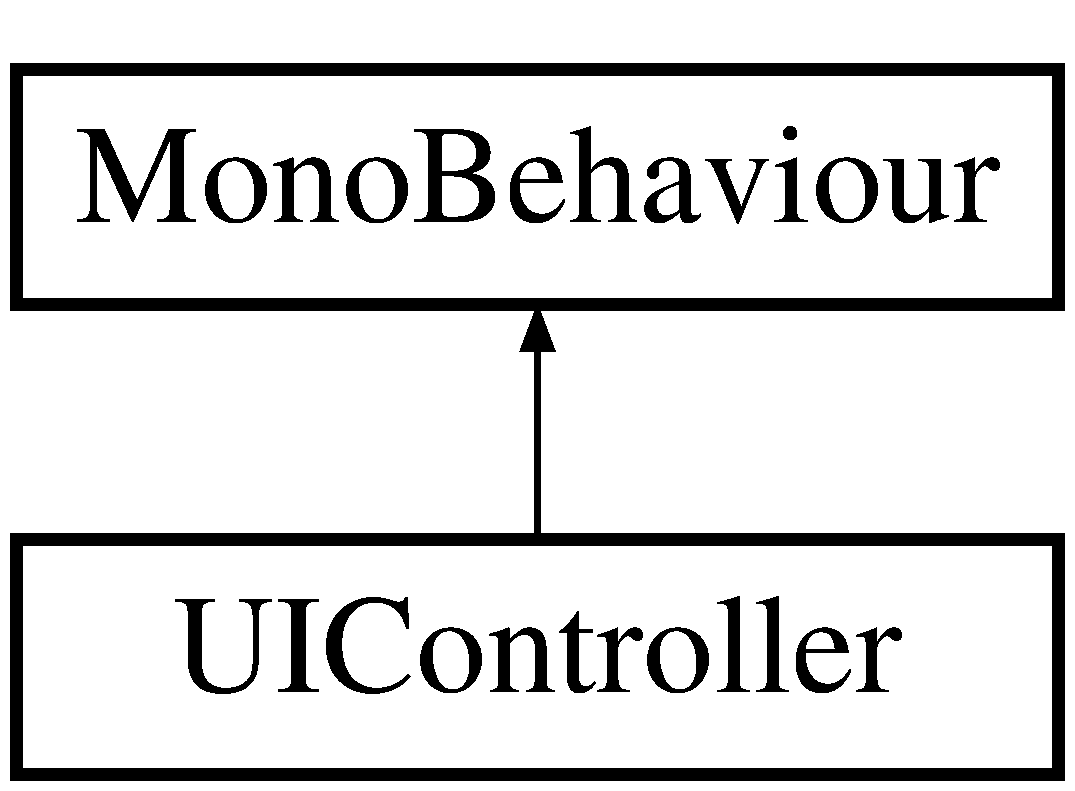
\includegraphics[height=2.000000cm]{class_u_i_controller}
\end{center}
\end{figure}
\subsection*{Private Member Functions}
\begin{DoxyCompactItemize}
\item 
\mbox{\Hypertarget{class_u_i_controller_a676b3b972c33885db4565ee43f23e459}\label{class_u_i_controller_a676b3b972c33885db4565ee43f23e459}} 
void {\bfseries Start} ()
\item 
\mbox{\Hypertarget{class_u_i_controller_adc5b0854a26bbcd71cc33274960bd0a9}\label{class_u_i_controller_adc5b0854a26bbcd71cc33274960bd0a9}} 
void {\bfseries Update} ()
\end{DoxyCompactItemize}
\subsection*{Private Attributes}
\begin{DoxyCompactItemize}
\item 
\mbox{\Hypertarget{class_u_i_controller_aac3690fd6f0e8307161343244e8ff125}\label{class_u_i_controller_aac3690fd6f0e8307161343244e8ff125}} 
\hyperlink{class_printer}{Printer} \hyperlink{class_u_i_controller_aac3690fd6f0e8307161343244e8ff125}{Printer}
\begin{DoxyCompactList}\small\item\em 
\begin{DoxyParams}{Parameters}
{\em \hyperlink{class_printer}{Printer}} & Object of the \hyperlink{class_printer}{Printer} that is used to request alot of settings of the printer (e.\+g. location, temperature).\\
\hline
\end{DoxyParams}
\end{DoxyCompactList}\item 
\mbox{\Hypertarget{class_u_i_controller_a1e06990406e89de41c6c8295ecd7870b}\label{class_u_i_controller_a1e06990406e89de41c6c8295ecd7870b}} 
Game\+Object \hyperlink{class_u_i_controller_a1e06990406e89de41c6c8295ecd7870b}{Printer\+Details}
\begin{DoxyCompactList}\small\item\em 
\begin{DoxyParams}{Parameters}
{\em Printer\+Details} & Game\+Object containing the textfields on the screen displaying the details of the printer (e.\+g. printer location, feedrate, bed height).\\
\hline
\end{DoxyParams}
\end{DoxyCompactList}\item 
\mbox{\Hypertarget{class_u_i_controller_a83aa464d971eff4f74cfb5891661693d}\label{class_u_i_controller_a83aa464d971eff4f74cfb5891661693d}} 
Text \hyperlink{class_u_i_controller_a83aa464d971eff4f74cfb5891661693d}{Extruder\+Temperature}
\begin{DoxyCompactList}\small\item\em 
\begin{DoxyParams}{Parameters}
{\em Extruder\+Temperature} & The text field for displaying the current extruder temperature.\\
\hline
\end{DoxyParams}
\end{DoxyCompactList}\item 
\mbox{\Hypertarget{class_u_i_controller_a680c68becba759ccd4b587406ab1c394}\label{class_u_i_controller_a680c68becba759ccd4b587406ab1c394}} 
Text \hyperlink{class_u_i_controller_a680c68becba759ccd4b587406ab1c394}{Bed\+Temperature}
\begin{DoxyCompactList}\small\item\em 
\begin{DoxyParams}{Parameters}
{\em Bed\+Temperature} & The text field for displaying the current bed temperature.\\
\hline
\end{DoxyParams}
\end{DoxyCompactList}\item 
\mbox{\Hypertarget{class_u_i_controller_a994f6e8efe28969227da85c0d0be9707}\label{class_u_i_controller_a994f6e8efe28969227da85c0d0be9707}} 
Text \hyperlink{class_u_i_controller_a994f6e8efe28969227da85c0d0be9707}{Feed\+Rate}
\begin{DoxyCompactList}\small\item\em 
\begin{DoxyParams}{Parameters}
{\em Feed\+Rate} & The text field for displaying the current feedrate.\\
\hline
\end{DoxyParams}
\end{DoxyCompactList}\item 
\mbox{\Hypertarget{class_u_i_controller_a5575def461bc517ce48b0de312c4ebd7}\label{class_u_i_controller_a5575def461bc517ce48b0de312c4ebd7}} 
Text \hyperlink{class_u_i_controller_a5575def461bc517ce48b0de312c4ebd7}{Extrusion\+Position}
\begin{DoxyCompactList}\small\item\em 
\begin{DoxyParams}{Parameters}
{\em Extrusion\+Position} & The text field for displaying the current position of the extruder.\\
\hline
\end{DoxyParams}
\end{DoxyCompactList}\item 
\mbox{\Hypertarget{class_u_i_controller_ac44230ef75e3b296750801393477de69}\label{class_u_i_controller_ac44230ef75e3b296750801393477de69}} 
Text \hyperlink{class_u_i_controller_ac44230ef75e3b296750801393477de69}{Extruder\+PositionX}
\begin{DoxyCompactList}\small\item\em 
\begin{DoxyParams}{Parameters}
{\em Extruder\+PositionX} & The text field for displaying the current x location of the print needle.\\
\hline
\end{DoxyParams}
\end{DoxyCompactList}\item 
\mbox{\Hypertarget{class_u_i_controller_a504b3ba6c916c43baba0df947dae89b5}\label{class_u_i_controller_a504b3ba6c916c43baba0df947dae89b5}} 
Text \hyperlink{class_u_i_controller_a504b3ba6c916c43baba0df947dae89b5}{Extruder\+PositionY}
\begin{DoxyCompactList}\small\item\em 
\begin{DoxyParams}{Parameters}
{\em Extruder\+PositionY} & The text field for displaying the current y location of the print needle.\\
\hline
\end{DoxyParams}
\end{DoxyCompactList}\item 
\mbox{\Hypertarget{class_u_i_controller_a49baeb13cde303094921023dbaa34910}\label{class_u_i_controller_a49baeb13cde303094921023dbaa34910}} 
Text \hyperlink{class_u_i_controller_a49baeb13cde303094921023dbaa34910}{Bed\+Height}
\begin{DoxyCompactList}\small\item\em 
\begin{DoxyParams}{Parameters}
{\em Bed\+Height} & The text field for displaying the current bed height.\\
\hline
\end{DoxyParams}
\end{DoxyCompactList}\item 
\mbox{\Hypertarget{class_u_i_controller_a08a3a7a00bc7bac76ac726a3735532eb}\label{class_u_i_controller_a08a3a7a00bc7bac76ac726a3735532eb}} 
Game\+Object \hyperlink{class_u_i_controller_a08a3a7a00bc7bac76ac726a3735532eb}{Simulation\+Details}
\begin{DoxyCompactList}\small\item\em 
\begin{DoxyParams}{Parameters}
{\em Simulation\+Details} & Game\+Object containing the textfields on the screen displaying the details of the simulation (e.\+g. filename, time speed of simulation).\\
\hline
\end{DoxyParams}
\end{DoxyCompactList}\item 
\mbox{\Hypertarget{class_u_i_controller_a2f5c3c69e83435b9b4c3a9cb5f3a75af}\label{class_u_i_controller_a2f5c3c69e83435b9b4c3a9cb5f3a75af}} 
Text \hyperlink{class_u_i_controller_a2f5c3c69e83435b9b4c3a9cb5f3a75af}{Time\+Multiplier}
\begin{DoxyCompactList}\small\item\em 
\begin{DoxyParams}{Parameters}
{\em Time\+Multiplier} & The text field for displaying the current time speed of the simulation.\\
\hline
\end{DoxyParams}
\end{DoxyCompactList}\item 
\mbox{\Hypertarget{class_u_i_controller_a30bd00985e2665fc0f4cda1a41df4ea4}\label{class_u_i_controller_a30bd00985e2665fc0f4cda1a41df4ea4}} 
Text \hyperlink{class_u_i_controller_a30bd00985e2665fc0f4cda1a41df4ea4}{File}
\begin{DoxyCompactList}\small\item\em 
\begin{DoxyParams}{Parameters}
{\em File} & The text field for displaying the current selected file to print from.\\
\hline
\end{DoxyParams}
\end{DoxyCompactList}\end{DoxyCompactItemize}


\subsection{Detailed Description}
This class updates the values that are displayed in an printer process. Things like details about the printer (e.\+g. print needle location, temperature) and simulation details (e.\+g. print time speed) are updated here. 



The documentation for this class was generated from the following file\+:\begin{DoxyCompactItemize}
\item 
C\+:/\+Users/\+Mission\+Mankind/\+Desktop/\+Scripts/U\+I\+Controller.\+cs\end{DoxyCompactItemize}

%--- End generated contents ---

% Index
\backmatter
\newpage
\phantomsection
\clearemptydoublepage
\addcontentsline{toc}{chapter}{Index}
\printindex

\end{document}
